%%%%%%%%%%%%%%%%%%%%%%%%%%%%%%%%%%%%%%%%%%%%%%%%%%%%%%%%%%%%%%%
%% OXFORD THESIS TEMPLATE

% Use this template to produce a standard thesis that meets the Oxford University requirements for DPhil submission
%
% Originally by Keith A. Gillow (gillow@maths.ox.ac.uk), 1997
% Modified by Sam Evans (sam@samuelevansresearch.org), 2007
% Modified by John McManigle (john@oxfordechoes.com), 2015
% Modified by Ulrik Lyngs (ulrik.lyngs@cs.ox.ac.uk), 2018, for use with R Markdown
%
% Ulrik Lyngs, 25 Nov 2018: Following John McManigle, broad permissions are granted to use, modify, and distribute this software
% as specified in the MIT License included in this distribution's LICENSE file.
%
% John tried to comment this file extensively, so read through it to see how to use the various options.  Remember
% that in LaTeX, any line starting with a % is NOT executed.  Several places below, you have a choice of which line to use
% out of multiple options (eg draft vs final, for PDF vs for binding, etc.)  When you pick one, add a % to the beginning of
% the lines you don't want.


%%%%% CHOOSE PAGE LAYOUT
% The most common choices should be below.  You can also do other things, like replacing "a4paper" with "letterpaper", etc.

% This one will format for two-sided binding (ie left and right pages have mirror margins; blank pages inserted where needed):
%\documentclass[a4paper,twoside]{templates/ociamthesis}
% This one will format for one-sided binding (ie left margin > right margin; no extra blank pages):
%\documentclass[a4paper]{ociamthesis}
% This one will format for PDF output (ie equal margins, no extra blank pages):
%\documentclass[a4paper,nobind]{templates/ociamthesis}
%UL 2 Dec 2018: pass this in from YAML
\documentclass[a4paper, nobind]{templates/ociamthesis}

% UL 5 January 2021 - add packages used by kableExtra
\usepackage{booktabs}
\usepackage{longtable}
\usepackage{array}
\usepackage{multirow}
\usepackage{wrapfig}
\usepackage{colortbl}
\usepackage{pdflscape}
\usepackage{tabu}
\usepackage{threeparttable}
\usepackage{threeparttablex}
\usepackage[normalem]{ulem}
\usepackage{makecell}
\usepackage[colorlinks=false,pdfpagelabels,hidelinks=true]{hyperref}
\usepackage{float}

%UL set section header spacing
\usepackage{titlesec}
% 
\titlespacing\subsubsection{0pt}{24pt plus 4pt minus 2pt}{0pt plus 2pt minus 2pt}

% UL 30 Nov 2018 pandoc puts lists in 'tightlist' command when no space between bullet points in Rmd file
\providecommand{\tightlist}{%
  \setlength{\itemsep}{0pt}\setlength{\parskip}{0pt}}
 
% UL 1 Dec 2018, fix to include code in shaded environments

%UL set whitespace around verbatim environments
\usepackage{etoolbox}
\makeatletter
\preto{\@verbatim}{\topsep=0pt \partopsep=0pt }
\makeatother

%UL 26 Mar 2019, enable strikethrough
\usepackage[normalem]{ulem}

%UL use soul package for correction highlighting
\usepackage{color, soul}
\usepackage{xcolor}
\definecolor{correctioncolor}{HTML}{CCCCFF}
\sethlcolor{correctioncolor}
\newcommand{\ctext}[3][RGB]{%
  \begingroup
  \definecolor{hlcolor}{#1}{#2}\sethlcolor{hlcolor}%
  \hl{#3}%
  \endgroup
}
\soulregister\ref7
\soulregister\cite7
\soulregister\autocite7
\soulregister\textcite7
\soulregister\pageref7

%%%%%%% PAGE HEADERS AND FOOTERS %%%%%%%%%
\usepackage{fancyhdr}
\setlength{\headheight}{15pt}
\fancyhf{} % clear the header and footers
\pagestyle{fancy}
\renewcommand{\chaptermark}[1]{\markboth{\thechapter. #1}{\thechapter. #1}}
\renewcommand{\sectionmark}[1]{\markright{\thesection. #1}} 
\renewcommand{\headrulewidth}{0pt}

\fancyhead[LO]{\emph{\leftmark}} 
\fancyhead[RE]{\emph{\rightmark}} 

% UL page number position 
\fancyfoot[C]{\emph{\thepage}} %regular pages
\fancypagestyle{plain}{\fancyhf{}\fancyfoot[C]{\emph{\thepage}}} %chapter pages

% JEM fix header on cleared pages for openright
\def\cleardoublepage{\clearpage\if@twoside \ifodd\c@page\else
   \hbox{}
   \fancyfoot[C]{}
   \newpage
   \if@twocolumn\hbox{}\newpage
   \fi
   \fancyhead[LO]{\emph{\leftmark}} 
   \fancyhead[RE]{\emph{\rightmark}} 
   \fi\fi}


%%%%% SELECT YOUR DRAFT OPTIONS
% This adds a "DRAFT" footer to every normal page.  (The first page of each chapter is not a "normal" page.)

% This highlights (in blue) corrections marked with (for words) \mccorrect{blah} or (for whole
% paragraphs) \begin{mccorrection} . . . \end{mccorrection}.  This can be useful for sending a PDF of
% your corrected thesis to your examiners for review.  Turn it off, and the blue disappears.
\correctionstrue

%%%%% BIBLIOGRAPHY SETUP
% Note that your bibliography will require some tweaking depending on your department, preferred format, etc.
% If you've not used LaTeX before, I recommend reading a little about biblatex/biber and getting started with it.
% If you're already a LaTeX pro and are used to natbib or something, modify as necessary.
% Either way, you'll have to choose and configure an appropriate bibliography format...


\usepackage[style=authoryear, sorting=nyt, backend=biber, maxcitenames=2, useprefix, doi=true, isbn=false, uniquename=false]{biblatex}
\newcommand*{\bibtitle}{Works Cited}

\addbibresource{references.bib}


% This makes the bibliography left-aligned (not 'justified') and slightly smaller font.
\renewcommand*{\bibfont}{\raggedright\small}


% Uncomment this if you want equation numbers per section (2.3.12), instead of per chapter (2.18):
%\numberwithin{equation}{subsection}


%%%%% THESIS / TITLE PAGE INFORMATION
% Everybody needs to complete the following:
\title{Bayesian spatio-temporal methods for small-area estimation of HIV indicators}
\author{Adam Howes}
\college{Department of Mathematics}

% Master's candidates who require the alternate title page (with candidate number and word count)
% must also un-comment and complete the following three lines:

% Uncomment the following line if your degree also includes exams (eg most masters):
%\renewcommand{\submittedtext}{Submitted in partial completion of the}
% Your full degree name.  (But remember that DPhils aren't "in" anything.  They're just DPhils.)
\degree{Doctor of Philosophy}
% Term and year of submission, or date if your board requires (eg most masters)
\degreedate{September 2023}


%%%%% YOUR OWN PERSONAL MACROS
% This is a good place to dump your own LaTeX macros as they come up.

\newcommand{\Sc}{\mathcal{S}}
\newcommand{\R}{\mathcal{R}}
\newcommand{\N}{\mathcal{N}}
\newcommand{\X}{\mathcal{X}} 
\newcommand{\m}{\mathbf{m}}
\newcommand{\bu}{\mathbf{u}}
\newcommand{\bv}{\mathbf{v}}
\newcommand{\w}{\mathbf{w}}
\newcommand{\x}{\mathbf{x}}
\newcommand{\y}{\mathbf{y}}
\newcommand{\z}{\mathbf{z}}
\newcommand{\bb}{\mathbf{b}}
\newcommand{\Hb}{\mathbf{H}}
\newcommand{\bphi}{\bm{\phi}}
\newcommand{\brho}{\bm{\rho}}
\newcommand{\btheta}{\bm{\theta}}
\newcommand{\bmeta}{\bm{\eta}}
\newcommand{\bvartheta}{\bm{\vartheta}}
\newcommand{\bmu}{\bm{\mu}}

\newcommand{\cmark}{\ding{51}}
\newcommand{\xmark}{\ding{55}}

\usepackage{amsmath}
\DeclareMathOperator*{\argmin}{arg\,min}
\DeclareMathOperator*{\argmax}{arg\,max}

\RequirePackage{bm}

% To make text superscripts shortcuts
	\renewcommand{\th}{\textsuperscript{th}} % ex: I won 4\th place
	\newcommand{\nd}{\textsuperscript{nd}}
	\renewcommand{\st}{\textsuperscript{st}}
	\newcommand{\rd}{\textsuperscript{rd}}

%%%%% THE ACTUAL DOCUMENT STARTS HERE
\begin{document}

%%%%% CHOOSE YOUR LINE SPACING HERE
% This is the official option.  Use it for your submission copy and library copy:
\setlength{\textbaselineskip}{22pt plus2pt}
% This is closer spacing (about 1.5-spaced) that you might prefer for your personal copies:
%\setlength{\textbaselineskip}{18pt plus2pt minus1pt}

% You can set the spacing here for the roman-numbered pages (acknowledgements, table of contents, etc.)
\setlength{\frontmatterbaselineskip}{17pt plus1pt minus1pt}

% UL: You can set the line and paragraph spacing here for the separate abstract page to be handed in to Examination schools
\setlength{\abstractseparatelineskip}{13pt plus1pt minus1pt}
\setlength{\abstractseparateparskip}{0pt plus 1pt}

% UL: You can set the general paragraph spacing here - I've set it to 2pt (was 0) so
% it's less claustrophobic
\setlength{\parskip}{2pt plus 1pt}

%
% Oxford University logo on title page
%
\def\crest{{
\includegraphics{templates/ic-small.pdf}}}
\renewcommand{\university}{Imperial College London}
\renewcommand{\submittedtext}{In partial fulfillment of the requirements for the degree of}


% Leave this line alone; it gets things started for the real document.
\setlength{\baselineskip}{\textbaselineskip}


%%%%% CHOOSE YOUR SECTION NUMBERING DEPTH HERE
% You have two choices.  First, how far down are sections numbered?  (Below that, they're named but
% don't get numbers.)  Second, what level of section appears in the table of contents?  These don't have
% to match: you can have numbered sections that don't show up in the ToC, or unnumbered sections that
% do.  Throughout, 0 = chapter; 1 = section; 2 = subsection; 3 = subsubsection, 4 = paragraph...

% The level that gets a number:
\setcounter{secnumdepth}{2}
% The level that shows up in the ToC:
\setcounter{tocdepth}{1}


%%%%% ABSTRACT SEPARATE
% This is used to create the separate, one-page abstract that you are required to hand into the Exam
% Schools.  You can comment it out to generate a PDF for printing or whatnot.

% JEM: Pages are roman numbered from here, though page numbers are invisible until ToC.  This is in
% keeping with most typesetting conventions.
\begin{romanpages}

% Title page is created here
\maketitle

%%%%% COPYRIGHT -- added by ATH.
\begin{copyrights}
  The copyright of this thesis rests with the author. Unless otherwise indicated, its contents are licensed under a Creative Commons Attribution-Non Commercial 4.0 International Licence (CC BY-NC).
  Under this licence, you may copy and redistribute the material in any medium or format. You may also create and distribute modified versions of the work.
  This is on the condition that: you credit the author and do not use it, or any derivative works, for a commercial purpose.
  When reusing or sharing this work, ensure you make the licence terms clear to others by naming the licence and linking to the licence text.
  Where a work has been adapted, you should indicate that the work has been changed and describe those changes.
  Please seek permission from the copyright holder for uses of this work that are not included in this licence or permitted under UK Copyright Law.
\end{copyrights}

%%%%% ORIGINALITY -- added by ATH.
\begin{originality}
  This thesis, and the work presented in it, is work that I conducted myself.
  In all cases where I describe others' work, I provide appropriate references.
\end{originality}

%%%%% DEDICATION -- If you'd like one, un-comment the following.
\begin{dedication}
  \textit{For someone, or something}
\end{dedication}

%%%%% ACKNOWLEDGEMENTS -- Nothing to do here except comment out if you don't want it.
\begin{acknowledgements}
 	Thanks to Seth Flaxman and Jeff Eaton for supervision of this research;
 staff and students of the StatML CDT at Imperial and Oxford;
 members of the HIV Inference Group at Imperial;
 members of the Machine Learning and Global Health Network;
 the Bill \& Melinda Gates Foundation and EPSRC for funding this PhD;
 Mike McLaren, Kevin Esvelt, the Nucleic Acid Observatory team, and the Sculpting Evolution lab for hosting my visit to the MIT Media Lab;
 Alex Stringer for hosting my visit to Waterloo;
 the Effective Altruism community;
 my friends and family.

 \begin{flushright}
 Adam Howes \\
 Imperial College London\\
 September 2023
 \end{flushright}
\end{acknowledgements}

%%%%% ABSTRACT -- Nothing to do here except comment out if you don't want it.
\begin{abstract}
	Progress towards ending AIDS as a public health threat by 2030 is faltering.
Effective public health response requires accurate, timely, high-resolution estimates of epidemic and demographic indicators.
Limitations of available data make obtaining such estimates difficult.
I develop and apply Bayesian spatio-temporal methods to meet this challenge.
Firstly, I examine models for area-level spatial structure.
Secondly, I estimate district-level HIV risk group proportions, enabling behavioural prioritisation of prevention services, as put forward by the Global AIDS Strategy.
Finally, I develop a novel Bayesian inference method, combining adaptive Gauss-Hermite quadrature with principal component analysis, motivated by the Naomi district-level model of HIV indicators.
Together, the contributions in this thesis help to guide precision HIV policy in sub-Saharan Africa, as well as advancing Bayesian methods for spatio-temporal data.
\end{abstract}

%%%%% MINI TABLES
% This lays the groundwork for per-chapter, mini tables of contents.  Comment the following line
% (and remove \minitoc from the chapter files) if you don't want this.  Un-comment either of the
% next two lines if you want a per-chapter list of figures or tables.
  \dominitoc % include a mini table of contents

% This aligns the bottom of the text of each page.  It generally makes things look better.
\flushbottom

% This is where the whole-document ToC appears:
\tableofcontents

\listoffigures
	\mtcaddchapter
  	% \mtcaddchapter is needed when adding a non-chapter (but chapter-like) entity to avoid confusing minitoc

% Uncomment to generate a list of tables:
\listoftables
  \mtcaddchapter
%%%%% LIST OF ABBREVIATIONS
% This example includes a list of abbreviations.  Look at text/abbreviations.tex to see how that file is
% formatted.  The template can handle any kind of list though, so this might be a good place for a
% glossary, etc.
%tibble(
%  Term = c("HIV"),
%  Abbreviation = C("Human Immunodeficiency Virus")
%  ) %>%
%  arrange(Term) %>%
%  kable(booktab = TRUE, escape = FALSE, "latex")

% After writing, reorder these as they appear in the text

% First parameter can be changed eg to "Glossary" or something.
% Second parameter is the max length of bold terms.
\begin{mclistof}{List of Abbreviations}{3.2cm}

\item[HIV] Human Immunodeficiency Virus.
\item[DALY] Disability Adjusted Life Year.
\item[AIDS] Acquired ImmunoDeficiency Syndrome.
\item[UNAIDS] The Joint United Nations Programme on HIV/AIDS.
\item[PEPFAR] President’s Emergency Plan for AIDS Relief.
\item[Global Fund] Global Fund to Fight AIDS, Tuberculosis, and Malaria.
\item[HIV] Demographic and Health Surveys.
\item[AIS] AIDS Indicator Survey.
\item[PrEP] Pre-Exposure Prophylaxis.
\item[PEP] Post-Exposure Prophylaxis.
\item[FSW] Female Sex Worker(s).
\item[MSM] Men who have Sex with Men.
\item[PWID] People Who Inject Drugs.
\item[TGP] Transgender People
\item[ANC] Antenatal Clinic.
\item[CDC] Centers for Disease Control and Prevention.
\item[UAT] Unlinked Anonymous Testing.
\item[PMTCT] Prevention of Mother-to-Child Transmission.
\item[PLHIV] People Living with HIV.
\item[TaSP] Treatment as Prevention.
\item[STI] Sexually Transmitted Infection.
\item[ART] Antiretroviral Therapy.
\item[VMMC] Voluntary Medical Male Circumcision.
\item[DHS] Demographic and Health Surveys.
\item[PHIA] Population-based HIV Impact Assessment.
\item[SSA] Sub-Saharan Africa.

\item[DDC] Data Defect Correlation.
\item[MCMC] Markov Chain Monte Carlo.
\item[NUTS] No-U-Turn Sampler.
\item[VI] Variational Inference.
\item[INLA] Integrated Nested Laplace Approximation.
\item[GP] Gaussian Process.
\item[CAR] Conditionally Auto-regressive.
\item[ICAR] Intrinsic Conditionally Auto-regressive.
\item[SAE] Small-Area Estimation.
\item[GMRF] Gaussian Markov Random Field.
\item[HMC] Hamiltonian Monte Carlo.
\item[GMRF] Gauss-Markov Random Field.
\item[HMC] Hamiltonian Monte Carlo.
\item[LM] Linear Model.
\item[GLM] Generalised Linear Model.
\item[GLMM] Generalised Linear Mixed effects Model.
\item[LGM] Latent Gaussian Model.
\item[ELGM] Extended Latent Gaussian Model.
\item[BF] Bayes Factor.
\item[CPO] Conditional Predictive Ordinate.
\item[DIC] Deviance Information Criterion.
\item[BIC] Bayesian Information Criterion.
\item[WAIC] Watanabe-Akaike Information Criterion.
\item[SR] Scoring Rule.
\item[SPSR] Strictly Proper Scoring Rule.
\item[CRPS] Continuous Ranked Probability Score.
\item[LS] Log Score.
\item[PIT] Probability Integral Transform.
\item[ECDF] Empirical Cumulative Difference Function.
\item[ESS] Effective Sample Size.
\item[IID] Independent and Identically Distributed.
\item[PPL] Probabilistic Programming Language.
\item[CCD] Central Composite Design.
\item[EB] Empirical Bayes.
\item[AGHQ] Adaptive Gauss-Hermite Quadrature.

\end{mclistof} 


%%%%% LIST OF NOTATION
\begin{mclistof}{List of Notations}{3.2cm}

\item[$\rho$] HIV prevalence.
\item[$\lambda$] HIV incidence.
\item[$\alpha$] ART coverage.
\item[$\mathcal{S}$] Spatial study region $\mathcal{S} \subseteq \mathbb{R}^2$.
\item[$s \in \mathcal{S}$] Point location.
\item[$\mathcal{T}$] Temporal study period $\mathcal{T} \subseteq \mathbb{R}$.
\item[$t \in \mathcal{T}$] Time.
\item[$\y$] Data, a $n$-vector.
\item[$\bphi$] Parameters, a $d$-vector $(\phi_1, \ldots, \phi_d)$.
\item[$\x$] Latent field, a $N$-vector $(x_1, \ldots, x_N)$.
\item[$\btheta$] Hyperparameters, a $m$-vector $(\theta_1, \ldots, \theta_m)$.
\item[$x \sim p(x)$] $x$ is distributed according to $p(x)$.
\item[$A_i$] Areal unit.
\item[$A_i \sim A_j$] Adjacency between areal units.
\item[$\mathbf{H}$] Hessian matrix.
\item[$\mathbf{R}$] Structure matrix.
\item[$\mathbf{Q}$] Precision matrix.
\item[$\bm{\Sigma}$] Covariance matrix.
\item[$\mathcal{N}$] Gaussian distribution.
\item[$k: \mathcal{X} \times \mathcal{X} \to \mathbb{R}$] Kernel function on the space $\mathcal{X}$.
\item[$A_i \sim A_j$] Adjacency between areal units.
\item[$\mathcal{Q}$] A set of quadrature nodes.
\item[$\omega: \mathcal{Q} \to \mathbb{R}$] A quadrature weighting function.
\item[$\mathcal{Q}(m, k)$] Gauss-Hermite quadrature points in $m$ dimensions with $k$ nodes per dimension, constructed according to a product rule.

\end{mclistof} 

% The Roman pages, like the Roman Empire, must come to its inevitable close.
\end{romanpages}

%%%%% CHAPTERS
% Add or remove any chapters you'd like here, by file name (excluding '.tex'):
\flushbottom

% all your chapters and appendices will appear here
\hypertarget{introduction}{%
\chapter{Introduction}\label{introduction}}

\adjustmtc
\markboth{Introduction}{}

This thesis is about applied and methodological Bayesian statistics.
It is Bayesian in the sense that I use probability models to arrive at conclusions based on data.
It is applied and methodological in the sense that I am concerned with real world questions and the means to answer them.

The real world questions relate to surveillance of the HIV epidemic in sub-Saharan Africa.
Millions of people are impacted by HIV every year.
Quantifying the epidemic using statistics is an important part of the public health response, and the path towards disease control and elimination.

The data I use relate to people's answers to survey questions or use of healthcare facilities.
It has location in space and time which should be taken into account.
Spatio-temporal data, while diverse, has distinctive commonalities which make its collective study worthwhile.

Computation is an essential part of modern statistical practice.
Each project chapter is accompanied by code, hosted on GitHub.

\hypertarget{chapter-overview}{%
\section{Chapter overview}\label{chapter-overview}}

\begin{itemize}
\tightlist
\item
  Chapter \ref{hiv-aids}: I begin by providing background on the HIV/AIDS epidemic.
\item
  Chapter \ref{bayes-st}: I then introduce the statistical concepts and notation used throughout the thesis.
\item
  Chapter \ref{beyond-borders}: The prevailing model for spatial structure used in small-area estimation \autocite{besag1991bayesian} was designed with analysis of a grid of pixels in mind.
  In disease mapping, we work using the districts of a country, which are not a grid.
  I evaluate the practical consequences of this this concern \autocite{howes2023beyond}.
\item
  Chapter \ref{multi-agyw}: Adolescent girls and young women are a demographic group at disproportionate risk of HIV infection.
  The Global AIDS Strategy suggests prioritising interventions on the basis of behaviour to prevent the most new infections using available resources.
  I estimate the size of behavioural risk groups across priority countries to enable implementation of this strategy, and assess the potential benefits in terms of numbers of new infections prevented \autocite{howes2023spatio}.
\item
  Chapter \ref{naomi-aghq}: The Naomi small-area estimation model \autocite{eaton2021naomi} is used by countries to estimate district-level HIV indicators.
  Motivated by this model, I develop an approximate Bayesian inference method combining adaptive Gauss-Hermite quadrature with principal components analysis \autocite{howes2023fast}.
  I apply the method to data from Malawi, and analyse the consequences of inference method choice for policy relevant outcomes.
  Further, I open the door to a new class of fast, flexible, and accurate Bayesian inference algorithms.
\item
  Chapter \ref{conclusions}: I discuss avenues for future work, and my conclusions regarding the research.
\end{itemize}

Figure \ref{fig:chapter-flowchart} gives the dependency structure for the above chapters.
Though the presented order is recommended, Chapter \ref{beyond-borders}, Chapter \ref{multi-agyw} and Chapter \ref{naomi-aghq}) may be read in any order.

\begin{figure}

{\centering 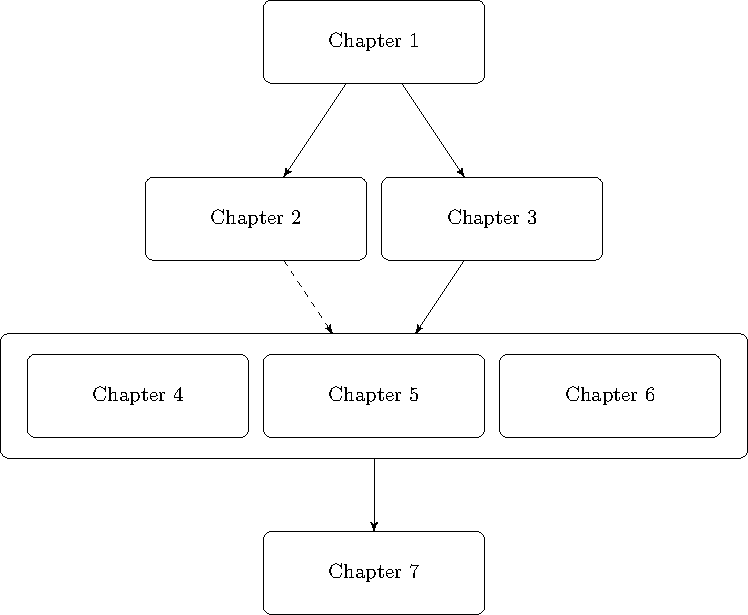
\includegraphics[width=0.95\linewidth]{figures/chapter-flowchart} 

}

\caption{Flowchart presenting the recommended chapter dependencies for this thesis. The dashed line represents a recommended, but not required dependency.}\label{fig:chapter-flowchart}
\end{figure}

\hypertarget{hiv-aids}{%
\chapter{The HIV/AIDS epidemic}\label{hiv-aids}}

\adjustmtc
\markboth{HIV/AIDS}{}

\hypertarget{background}{%
\section{Background}\label{background}}

Human immunodeficiency virus (HIV) is a retrovirus which infects humans.
If left untreated, a more advanced stage known as acquired immunodeficiency syndrome (AIDS) can develop.
HIV primarily attacks a type of white blood cell vital for the function of the immune system.
As a result, AIDS is characterised by increased risk of developing opportunistic infections.

HIV is transmitted by exposure to specific bodily fluids of an infected person.
The most common mode of transmission is through unprotected anal or vaginal sex.
Transmission can also occur from a mother to her baby, or when drug injection equipment is shared.

The first AIDS cases were reported in Los Angeles in the early 1980s.
Since then, HIV has spread globally, resulting in 40 million deaths.
A major international effort has been made to address the epidemic.
Large global health initiatives focused on HIV/AIDS include the Global Fund to Fight AIDS, Tuberculosis, and Malaria (GFATM; \$29.2 billion) and the President's Emergency Plan for AIDS Relief (PEPFAR; \$85 billion).

Significant progress has been made, both in reducing the yearly number of new HIV cases and decreasing the yearly number of HIV related deaths (Figure \ref{fig:overall-picture}).
This has been possible because of the following interventions:

\begin{itemize}
\tightlist
\item
  Antiretroviral therapy (ART) is a drug which stops the virus from replicating in the body.
  By taking ART daily, a person living with HIV can live a full and healthy life.
  There were 38 million people living with HIV in 2021, the majority of whom taking ART.
  ART has been estimated to have averted this many million deaths.
  Furthermore, if the virus is undetectable then it cannot be transmitted sexually.
  For this reason, treatment also operates as prevention (TaSP).
  ART has been estimated to have averted this many new infections.
\item
  Condoms are an inexpensive and effective method for prevention of HIV and other sexually transmitted infections (STIs).
  Scale-up of condom usage since 1990 has been estimated to have averted over 10 million new HIV infections \autocite{stover2021impact}.
\item
  Pre-exposure prophylaxis (PrEP) and post-exposure prophylaxis (PEP) are drugs which can be taken before and after exposure to prevent transmission.
\item
  Voluntary medical male circumcision (VMMC) has been found to provide partial protection against female-to-male HIV transmission.
\end{itemize}

\begin{figure}

{\centering 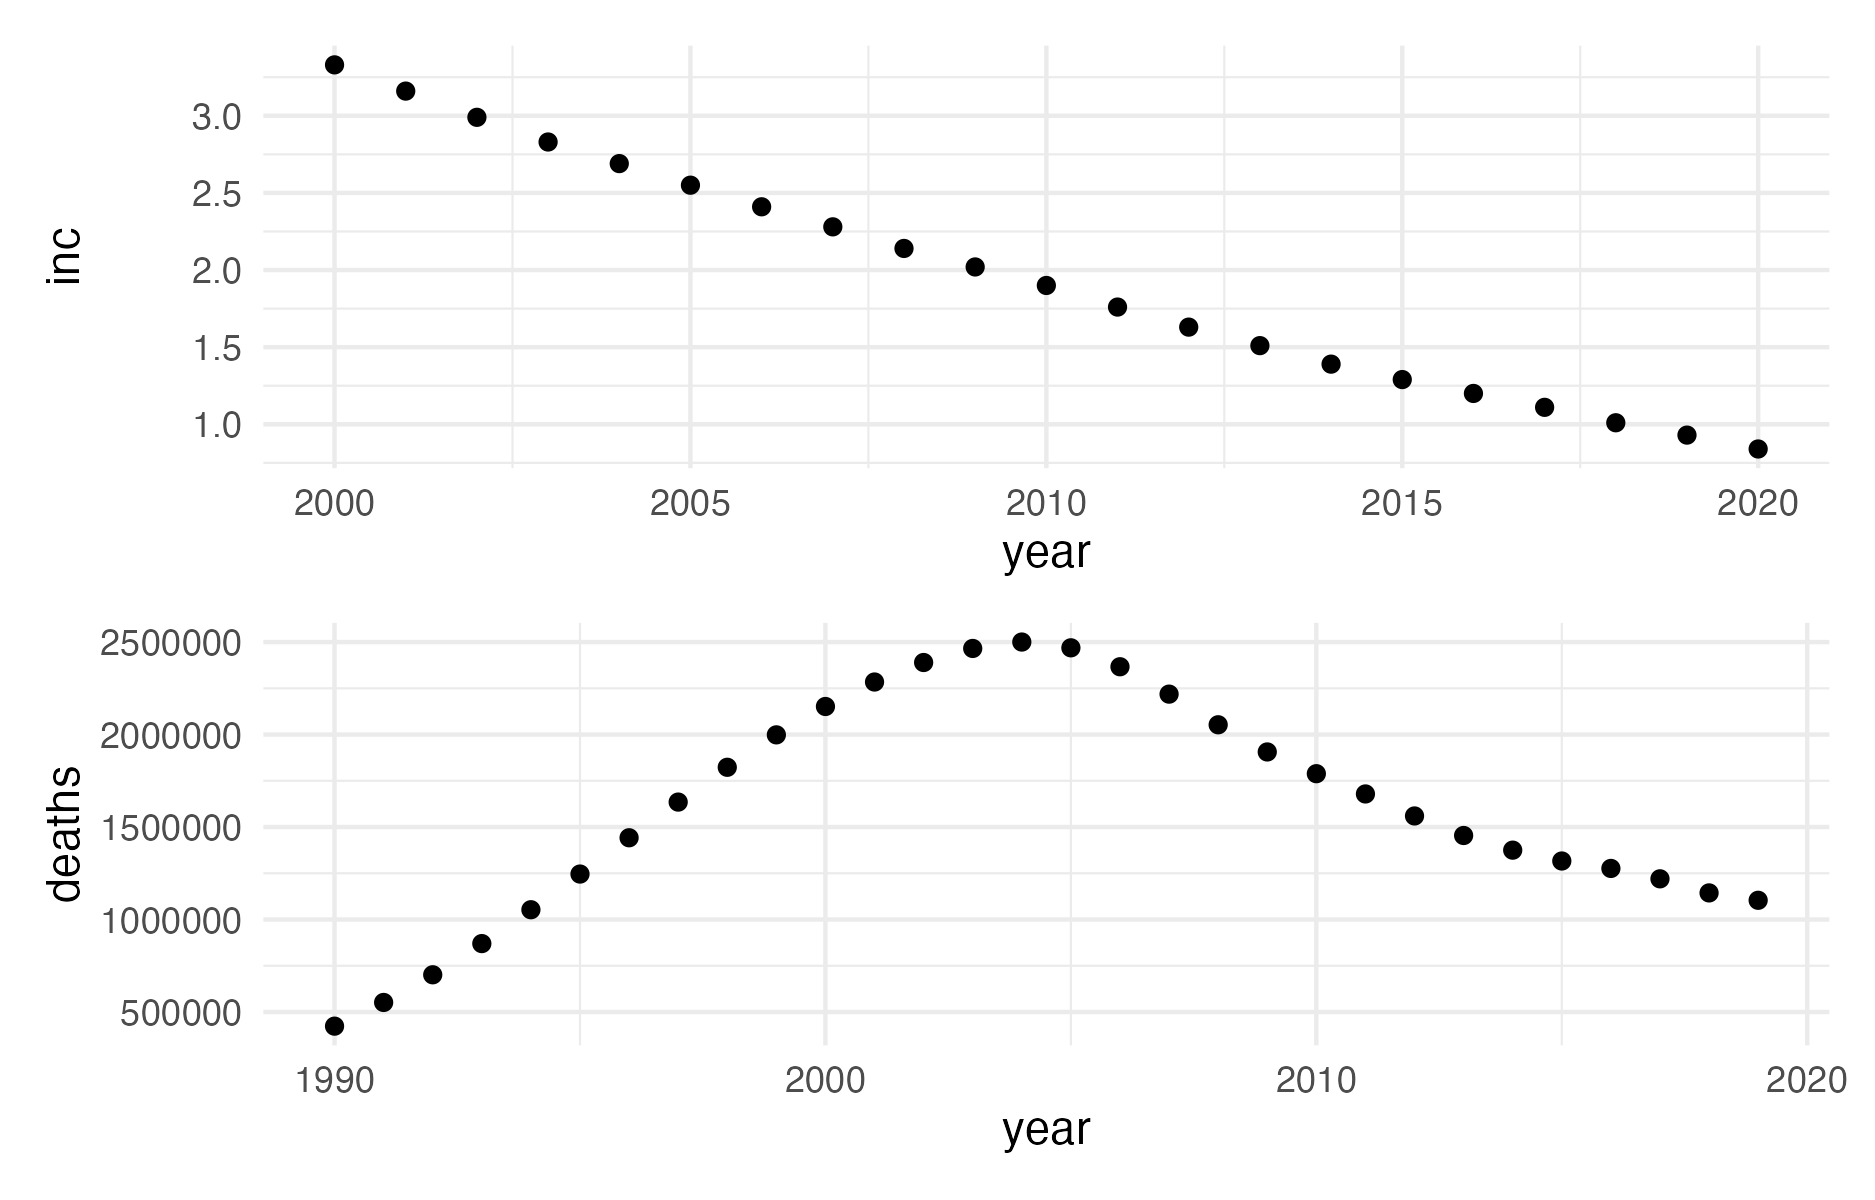
\includegraphics[width=0.95\linewidth]{figures/overall-picture} 

}

\caption{Overall picture.}\label{fig:overall-picture}
\end{figure}

In 2021 there were 650 thousand HIV related deaths and 1.5 million people newly infected with HIV \autocite{unaids2021global}.

There is substantial geographic inequality in disease burden.
In some countries, the epidemic is concentrated within small populations, and prevalence is low.
In others, transmission is sustained in the general population, and prevalence is higher.
Most of the countries severely affected by HIV are in sub-Saharan Africa (SSA), which accounts for this percentage of people living with HIV (PLHIV) worldwide.
There is also significant geographic variation within countries.

Across all settings, there is substantial inequality in disease burden between groups.
Groups at increased risk of HIV infection are known as key populations (KPs), and include men who have sex with men (MSM), female sex workers (FSW), people who inject drugs (PWID), and transgender people (TGP).
KPs are often marginalised, and face legal and social issues.

In SSA, risk is more diffuse than in concentrated settings.
Demographic groups, while not classified as KPs, at increased risk of HIV infection include adolescent girls and young women (AGYW), migratory populations, and rural communities.

HIV interventions should be prioritised to have the greatest impact on the epidemic.
The precision public health paradigm aims to get the right interventions, to the right populations, in the right place, at the right time.
This requires data.

\hypertarget{hiv-surveillance}{%
\section{HIV surveillance}\label{hiv-surveillance}}

HIV surveillance refers to the collection, analysis, interpretation and dissemination of data relating to HIV/AIDS.
Surveillance can used to track epidemic indicators, identify at-risk populations, find drivers of transmission, and evaluate the impact of prevention and treatment programs.
Important indicators include:

\begin{itemize}
\tightlist
\item
  \textbf{HIV prevalence} The proportion of the population who have HIV, typically given as a percentage;
\item
  \textbf{HIV incidence} The rate of new HIV infections, typically given as number of new infections per 1000 person years; and
\item
  \textbf{ART coverage} The proportion of PLHIV who are on ART, typically given as a percentage.
\end{itemize}

There are significant difficulties associated with obtaining estimates of these indicators, which are reliable, timely, and at an appropriate resolution.

\begin{enumerate}
\def\labelenumi{\arabic{enumi}.}
\tightlist
\item
  \textbf{Information sparsity}
  Collection of data is costly and time consuming.
  As a result, data may not be available for at the particular time and location of interest.
\item
  \textbf{Survey biases}
\item
  \textbf{Conflicting information}
\item
  \textbf{Hard to reach populations}
  Many of the key populations at greatest risk are difficult to reach
\item
  \textbf{Changing demographics}
\end{enumerate}

These limitations foreground the importance of statistical modelling.
Important modelling techniques include:

\begin{enumerate}
\def\labelenumi{\arabic{enumi}.}
\tightlist
\item
  \textbf{Borrowing information}
\item
  \textbf{Evidence synthesis}
\item
  \textbf{Expert guidance}
\end{enumerate}

Aims for HIV response going forward, and surveillance capabilities are needed to meet them.
Phasing out of nationally-representative household surveys for HIV.

\hypertarget{bayes-st}{%
\chapter{Bayesian spatio-temporal statistics}\label{bayes-st}}

\adjustmtc
\markboth{Bayesian}{}

\hypertarget{bayesian-statistics}{%
\section{Bayesian statistics}\label{bayesian-statistics}}

Bayesian statistics is a mathematical paradigm for learning from data.
I provide a brief overview in this section.
For a more complete introduction, I recommend \textcite{mcelreath2020statistical} or \textcite{gelman2013bayesian}.

\hypertarget{bayesian-modelling}{%
\subsection{Bayesian modelling}\label{bayesian-modelling}}

At its best, the Bayesian paradigm allows the analyst focus on how best to model the data.
This is achieved by the construction of a generative model \(p(\y, \bvartheta)\) for the observed data \(\y = (y_1, \ldots, y_n)\) together with parameters \(\bvartheta = (\vartheta_1, \ldots, \vartheta_d)\).
The model is generative in the sense that one can simulate from it to obtain draws \((\y, \bvartheta) \sim p(\y, \bvartheta)\).
If these draws differ too greatly from what the analyst would expect, then the generative model can be refined.
In this way, models can be built iteratively, and complexity added gradually.

The model is usually constructed from two parts, known as the likelihood \(p(\y \, | \, \bvartheta)\) and the prior \(p(\bvartheta)\) whereby \(p(\y, \bvartheta) = p(\y \, | \, \bvartheta) p(\bvartheta)\).
The likelihood, as a function of \(\bvartheta\) with \(\y\) fixed, reflects the probability of observing the data when the true value of the parameters is \(\bvartheta\).
The prior encapsulates beliefs about the parameters \(\bvartheta\) before the data is observed.
There has been substantial discussion and disagreement about how the prior should be specified.
That said, the distinction between likelihood and prior can sometimes be blurred (Section \ref{hierarchical-lgm-elgm}).
As such, it may be argued that these difficulties are not unique to the prior and ultimately the challenge of specifying the data generating process is better thought of more holistically \autocite{gelman2017prior}.

\hypertarget{bayesian-computation}{%
\subsection{Bayesian computation}\label{bayesian-computation}}

The posterior distribution \(p(\bvartheta \, | \, \y)\) represents beliefs about the parameters given the observed data.
Using the eponymous Bayes' theorem, it is given by
\begin{equation}
p(\bvartheta \, | \, \y) = \frac{p(\y \, | \, \bvartheta) p(\bvartheta)}{p(\y)}. \label{eq:posterior}
\end{equation}
Unfortunately, Equation \ref{eq:posterior} is usually intractable to calculate directly because of the integral \(p(\y) = \int p(\y, \bvartheta) \text{d}\bvartheta\) in the denominator.
As such, the typically situation is that although the numerator is proportional to the posterior \(p(\bvartheta \, | \, \y) \propto p(\y \, | \, \bvartheta) p(\bvartheta)\) and easy to evaluate, it is not easy to evaluate the posterior itself.

A great variety of computational methods have been developed which aim to tackle this problem.
Markov chain Monte Carlo (MCMC) is the most popular approach, and proceeds by simulating samples from a Markov chain with the posterior as its stationary distribution.
Variational Bayes approaches assume the posterior distribution belongs to a certain class of functions and use optimisation to choose the best member of that class.

\hypertarget{interplay-between-modelling-and-computation}{%
\subsection{Interplay between modelling and computation}\label{interplay-between-modelling-and-computation}}

Bayesian computation aspires to abstract away calculation of the posterior distribution from the analyst.
Modern computational techniques and software have made this aspiration a reality for many models.
However, computation of the posterior remains intractable for a substantial majority of models.
As such, the analyst need not only to be concerned with choosing a model suitable for the data, but also choosing a model for which the posterior is tractable in reasonable time.
It is in this sense, that there is an interplay between modelling and computation.
As computation improves, the space of models available to the analyst expands.

\hypertarget{spatio-temporal-statistics}{%
\section{Spatio-temporal statistics}\label{spatio-temporal-statistics}}

In spatio-temporal statistics \autocite{cressie2015statistics} we observe data indexed by spatial or temporal location.
In this thesis we assume that the spatial study region \(\mathcal{S} \subseteq \mathbb{R}^2\) has two dimensions, corresponding to latitude and longitude.
Data may be associated to a point \(s \in \mathcal{S}\) or area \(A \subseteq \mathcal{S}\) in the study region.
The temporal study period \(\mathcal{T} \subseteq \mathbb{R}\) can more generally be assumed to be one dimensional.

Correlation structure is an important feature of spatio-temporal data.

\hypertarget{small-area-estimation}{%
\section{Small-area estimation}\label{small-area-estimation}}

\hypertarget{hierarchical-lgm-elgm}{%
\section{Model classes}\label{hierarchical-lgm-elgm}}

\hypertarget{hierarchical}{%
\subsection{Hierarchical models}\label{hierarchical}}

Real world data usually has hierarchical structure.
For example, there might be multiple measurements of the same unit (Figure \ref{fig:hierarchical-structure}).

Bayesian hierarchical models are comprised of multiple stages.
For example in a three-stage model, we have
\begin{align}
\y &\sim p(\y \, | \, \x, \btheta), \\
\x &\sim p(\x \, | \, \btheta), \\
\btheta &\sim p(\btheta),
\end{align}
with posterior proportional to \(p(\x, \btheta \, | \, \y) \propto p(\y \, | \, \x, \btheta) p(\x \, | \, \btheta) p(\btheta)\).

\begin{figure}

{\centering 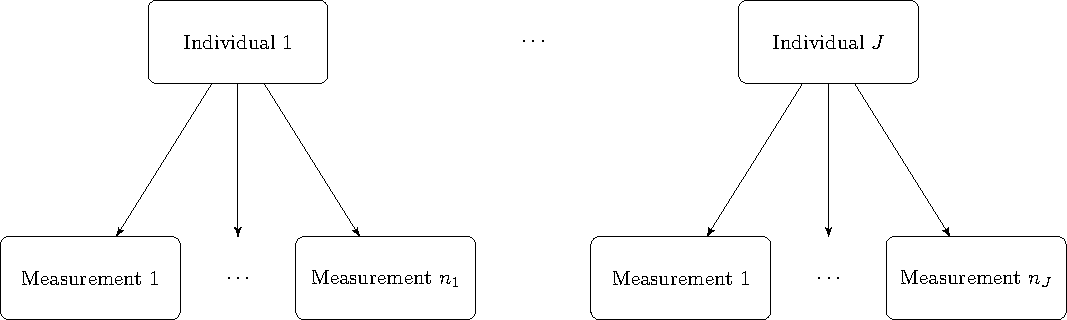
\includegraphics[width=0.95\linewidth]{figures/hierarchical-structure} 

}

\caption{Data often has a hierarchical structure.}\label{fig:hierarchical-structure}
\end{figure}

\hypertarget{latent-gaussian-models}{%
\subsection{Latent Gaussian models}\label{latent-gaussian-models}}

Latent Gaussian models {[}LGMs; \textcite{rue2009approximate}{]} are a class of three-stage Bayesian hierarchical models in which, loosely speaking, the middle layer is Gaussian.
More specifically, in an LGM, the likelihood is given by
\begin{align*}
y_i &\sim p(y_i \, | \, \eta_i, \theta_1), \quad i \in [n]\\
\mu_i &= \mathbb{E}(y_i \, | \, \eta_i) = g(\eta_i), \\
\eta_i &= \beta_0 + \sum_{l = 1}^{p} \beta_j z_{ji} + \sum_{k = 1}^{r} f_k(u_{ki}),
\end{align*}
where \([n] = \{1, \ldots, n\}\).
The response variable is \(\y = (y)_{i \in [n]}\) with likelihood \(p(\y \, | \, \bmeta, \btheta_1) = \prod_{i = 1}^n p(y_i \, | \, \eta_i, \btheta_1)\), where \(\bmeta = (\eta)_{i \in [n]}\).
Each response has conditional mean \(\mu_i\) with inverse link function \(g: \mathbb{R} \to \mathbb{R}\) such that \(\mu_i = g(\eta_i)\).
The vector \(\btheta_1 \in \mathbb{R}^{s_1}\), with \(s_1\) assumed small, are additional parameters of the likelihood.
The structured additive predictor \(\eta_i\) may include an intercept \(\beta_0\), linear effects \(\beta_j\) of the covariates \(z_{ji}\), and unknown functions \(f_k(\cdot)\) of the covariates \(u_{ki}\).
The parameters \(\beta_0\), \(\{\beta_j\}\), \(\{f_k(\cdot)\}\) are each assigned Gaussian priors, and can be collected into a vector \(\x \in \mathbb{R}^N\) such that \(\x \sim \mathcal{N}(\mathbf{0}, \mathbf{Q}(\btheta_2)^{-1})\) where \(\btheta_2 \in \mathbb{R}^{s_2}\) are further parameters, again with \(s_2\) assumed small.
Let \(\btheta = (\btheta_1, \btheta_2) \in \mathbb{R}^m\) with \(m = s_1 + s_2\) be all hyperparameters, with prior \(p(\btheta)\).
In total, the parameters of the LGM \(\bvartheta = (\x, \btheta)\) comprise both the latent field and hyperparameters.

Spatio-temporal data are well suited to being modelled with LGMs.

\hypertarget{extended-latent-gaussian-models}{%
\subsection{Extended latent Gaussian models}\label{extended-latent-gaussian-models}}

Some leading-edge spatio-temporal models used in small-area estimation fall outside the LGM class.
However, many of these models do fit into the class of extended latent Gaussian models (ELGMs) as proposed by \textcite{stringer2021fast}.
By allowing many-to-one link functions, ELGMs facilitate modelling of non-linearities.
In particular, the structured additive predictor is redefined as \(\bmeta = (\eta)_{i \in [N_n]}\), where \(N_n \in \mathbb{N}\) is a function of \(n\), and it is possible that \(N_n \neq n\).
Each mean response \(\mu_i\) now depends on some subset \(\mathcal{J}_i \subseteq [N_n]\) of indices of \(\bmeta\), with \(\cup_{i = 1}^n \mathcal{J}_i = [N_n]\) and \(1 \leq |\mathcal{J}_i| \leq N_n\).
The inverse link function \(g(\cdot)\) is redefined for each observation to be a possibly many-to-one mapping \(g_i: \mathbb{R}^{|\mathcal{J}_i|} \to \mathbb{R}\), such that \(\mu_i = g_i(\bmeta_{\mathcal{J}_i})\).
Put together, ELGMs are then of the form
\begin{align*}
y_i &\sim p(y_i \, | \, \bmeta_{\mathcal{J}_i}, \btheta_1), \quad i \in [n] \\
\mu_i &= \mathbb{E}(y_i \, | \, \bmeta_{\mathcal{J}_i}) = g_i(\bmeta_{\mathcal{J}_i}), \\
\eta_j &= \beta_0 + \sum_{l = 1}^{p} \beta_j z_{ji} + \sum_{k = 1}^{r} f_k(u_{ki}), \quad j \in [N_n],
\end{align*}
with latent field and hyperparameter priors as in the LGM case.

Instances of ELGM structures being useful for small-area estimation are as follows.

\hypertarget{beyond-borders}{%
\chapter{Spatial structure}\label{beyond-borders}}

\adjustmtc
\markboth{Models for spatial structure}{}

In this chapter, I describe an investigation of spatial random effects specifications.
The motivated for this investigation was one of the fundamental questions encountered by an analyst during model construction.
Namely, should the model be augmented to better capture a feature of the data generating process that we believe exists?
The results are presented in \textcite{howes2023beyond}.

Code for the analysis in this chapter is available from \href{https://github.com/athowes/beyond-borders}{\texttt{athowes/beyond-borders}} and supported by the R package \href{https://athowes.github.io/arealutils}{\texttt{arealutils}}.

\hypertarget{background-1}{%
\section{Background}\label{background-1}}

\hypertarget{areal-and-point-data}{%
\subsection{Areal and point data}\label{areal-and-point-data}}

\hypertarget{spatial-random-effects}{%
\subsection{Spatial random effects}\label{spatial-random-effects}}

\hypertarget{models-based-on-adjacency}{%
\section{Models based on adjacency}\label{models-based-on-adjacency}}

\hypertarget{the-besag-model}{%
\subsection{The Besag model}\label{the-besag-model}}

\hypertarget{the-bym2-model}{%
\subsection{The BYM2 model}\label{the-bym2-model}}

\hypertarget{models-using-kernels}{%
\section{Models using kernels}\label{models-using-kernels}}

\hypertarget{the-centroid-kernel-model}{%
\subsection{The centroid kernel model}\label{the-centroid-kernel-model}}

\hypertarget{the-integrated-kernel-model}{%
\subsection{The integrated kernel model}\label{the-integrated-kernel-model}}

\hypertarget{simulation-study}{%
\section{Simulation study}\label{simulation-study}}

\hypertarget{synthetic-data-sets}{%
\subsection{Synthetic data-sets}\label{synthetic-data-sets}}

\hypertarget{inferential-models}{%
\subsection{Inferential models}\label{inferential-models}}

\hypertarget{priors}{%
\subsubsection{Priors}\label{priors}}

\hypertarget{kernel-details}{%
\subsubsection{Kernel details}\label{kernel-details}}

\hypertarget{inference-algorithms}{%
\subsection{Inference algorithms}\label{inference-algorithms}}

\hypertarget{model-assessment}{%
\subsection{Model assessment}\label{model-assessment}}

\hypertarget{continuous-ranked-probability-score}{%
\subsubsection{Continuous ranked probability score}\label{continuous-ranked-probability-score}}

\hypertarget{results}{%
\subsection{Results}\label{results}}

\hypertarget{hiv-prevalence-study}{%
\section{HIV prevalence study}\label{hiv-prevalence-study}}

\hypertarget{results-1}{%
\subsection{Results}\label{results-1}}

\hypertarget{discussion}{%
\section{Discussion}\label{discussion}}

\hypertarget{limitations}{%
\subsection{Limitations}\label{limitations}}

\hypertarget{conclusion}{%
\subsection{Conclusion}\label{conclusion}}

\hypertarget{multi-agyw}{%
\chapter{A model for risk group proportions}\label{multi-agyw}}

\adjustmtc
\markboth{A model for risk group proportions}{}

In this chapter I describe an application of Bayesian spatio-temporal statistics to small-area estimation of HIV risk group proportions.
This work was conducted in collaboration with colleagues from the MRC Centre for Global Infectious Disease Analysis and UNAIDS.
My primary role was to develop the statistical model.
I built on an earlier version of the analysis conducted by Kathryn Risher.
The results are presented in \textcite{howes2023spatio}.
Kathryn has also created a spreadsheet tool using the estimates which is now being used by countries to guide policy.
Code for the analysis in this chapter is available from \href{https://github.com/athowes/multi-agyw}{\texttt{athowes/multi-agyw}} and supported by the R package \href{https://athowes.github.io/multi.utils}{\texttt{multi.utils}} \autocite{multiutils}.

\hypertarget{background-2}{%
\section{Background}\label{background-2}}

Adolescent girls and young women (AGYW, defined here as females aged 15-29) are a demographic group at increased risk of HIV infection.
Though AGHYW are only 28\% of the population, they comprise 44\% of new infections \autocite{unaids2021update}.
HIV incidence for AGYW is 2.4 times higher than for similarly aged males.
The social and biological reasons for this disparity are given in Table \ref{tab:agyw-reasons}.

\begin{longtable}[]{@{}
  >{\raggedright\arraybackslash}p{(\columnwidth - 2\tabcolsep) * \real{0.5000}}
  >{\raggedright\arraybackslash}p{(\columnwidth - 2\tabcolsep) * \real{0.5000}}@{}}
\caption{\label{tab:agyw-reasons} AYGW are at higher risk of HIV infection for interacting social and biological reasons.}\tabularnewline
\toprule\noalign{}
\begin{minipage}[b]{\linewidth}\raggedright
Reason
\end{minipage} & \begin{minipage}[b]{\linewidth}\raggedright
Description
\end{minipage} \\
\midrule\noalign{}
\endfirsthead
\toprule\noalign{}
\begin{minipage}[b]{\linewidth}\raggedright
Reason
\end{minipage} & \begin{minipage}[b]{\linewidth}\raggedright
Description
\end{minipage} \\
\midrule\noalign{}
\endhead
\bottomrule\noalign{}
\endlastfoot
Structural vulnerability and power imbalances & Gender inequality, lack of agency, economic factors, limited healthcare access, stigma and discrimination \\
Age patterns of sexual mixing & Older male partners have higher prevalence of HIV \\
Younger age at first sex & Text \\
Increased susceptibility to HIV infection & Immature reproductive tract, including a thinner cervical lining and higher levels of immune cells \\
\end{longtable}

On this basis, AGYW have been identified as a priority population for HIV prevention services \autocite{saul2018dreams,global2018measurement}.
The Global AIDS Strategy 2021-2026 \autocite{unaids2021global} proposed stratifying HIV prevention packages to AGYW based on 1) local population-level HIV incidence and 2) individual-level sexual risk behaviour.
As risk depends on both factors, prioritisation of prevention services would be more efficient if both are taken into account (Figure \ref{fig:risk-grid}).
The strategy encourages programmes to define targets for the proportion of AGYW to be reached with a range of interventions.
Estimates of the size of each risk group are required.

\begin{figure}

{\centering 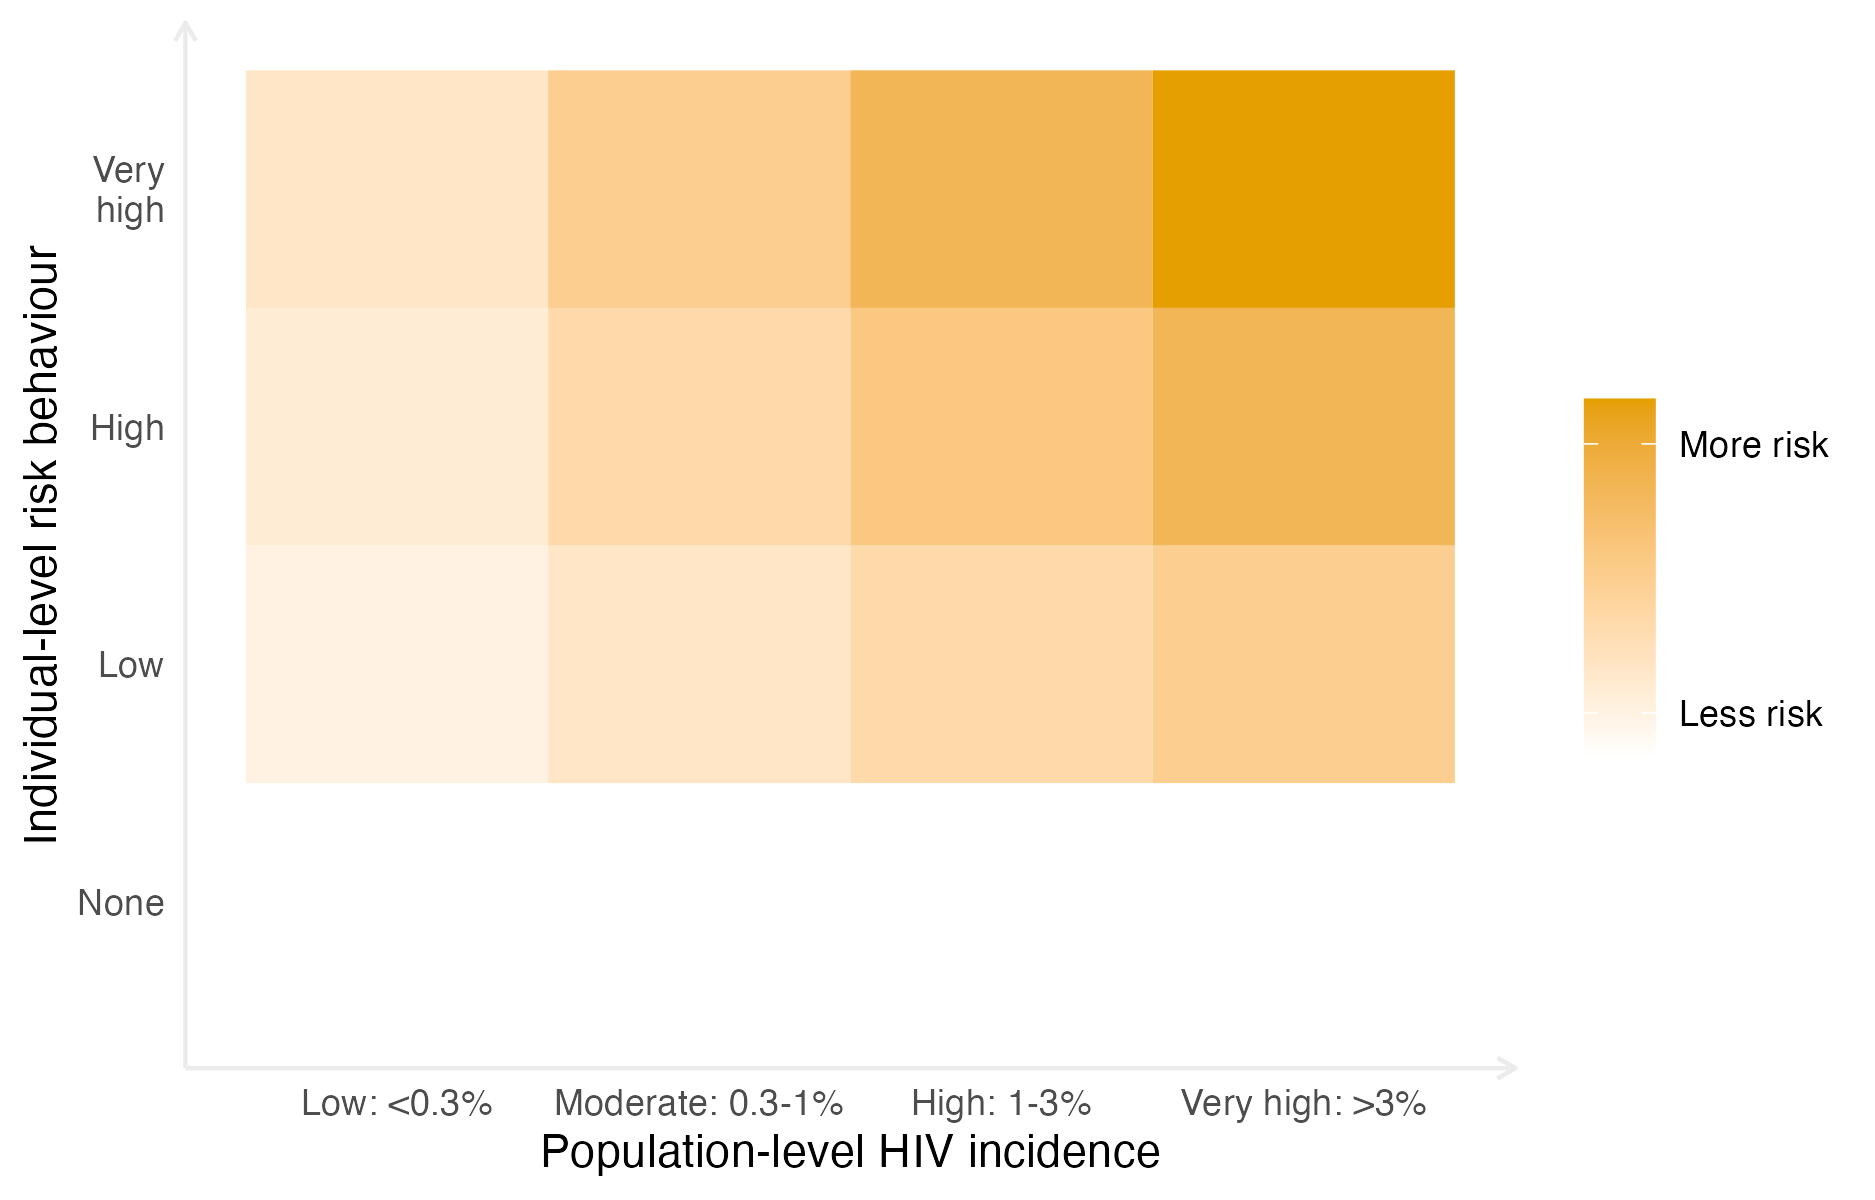
\includegraphics[width=0.95\linewidth]{figures/risk-grid} 

}

\caption{Risk depends on both individual-level risk behaviour and population-level HIV incidence.}\label{fig:risk-grid}
\end{figure}

\begin{longtable}[]{@{}
  >{\raggedright\arraybackslash}p{(\columnwidth - 6\tabcolsep) * \real{0.1818}}
  >{\raggedright\arraybackslash}p{(\columnwidth - 6\tabcolsep) * \real{0.2000}}
  >{\raggedright\arraybackslash}p{(\columnwidth - 6\tabcolsep) * \real{0.3455}}
  >{\raggedright\arraybackslash}p{(\columnwidth - 6\tabcolsep) * \real{0.2727}}@{}}
\caption{\label{tab:risk-groups} Behavioural risk groups.}\tabularnewline
\toprule\noalign{}
\begin{minipage}[b]{\linewidth}\raggedright
Risk group
\end{minipage} & \begin{minipage}[b]{\linewidth}\raggedright
Description
\end{minipage} & \begin{minipage}[b]{\linewidth}\raggedright
Local HIV incidence
\end{minipage} & \begin{minipage}[b]{\linewidth}\raggedright
Incidence ratio
\end{minipage} \\
\midrule\noalign{}
\endfirsthead
\toprule\noalign{}
\begin{minipage}[b]{\linewidth}\raggedright
Risk group
\end{minipage} & \begin{minipage}[b]{\linewidth}\raggedright
Description
\end{minipage} & \begin{minipage}[b]{\linewidth}\raggedright
Local HIV incidence
\end{minipage} & \begin{minipage}[b]{\linewidth}\raggedright
Incidence ratio
\end{minipage} \\
\midrule\noalign{}
\endhead
\bottomrule\noalign{}
\endlastfoot
None & Not sexually active & -- & 0.0 \\
Low & One cohabiting partner & -- & 1.0 (Baseline) \\
High & Non-regular or multiple partner(s) & -- & 1.72 \\
Very High & Transactional sex (adjusted to correspond to female sex workers) & 0.1-0.3\% & 13.0 \\
& & 0.3-1.0\% & 9.0 \\
& & 1.0-3.0\% & 6.0 \\
& & \textgreater3.0\% & 3.0 \\
\end{longtable}

\hypertarget{data}{%
\section{Data}\label{data}}

I used household survey data from 13 designated AGYW priority countries.: Botswana, Cameroon, Kenya, Lesotho, Malawi, Mozambique, Namibia, South Africa, Eswatini, Tanzania, Uganda, Zambia and Zimbabwe.

For each survey, I classified respondents into one of four behavioural risk groups according to reported sexual risk behaviour in the past 12 months.
These risk groups were:

\begin{enumerate}
\def\labelenumi{\arabic{enumi}.}
\tightlist
\item
  Not sexually active
\item
  One cohabiting sexual partner
\item
  Non-regular or multiple sexual partner(s), and
\item
  AGYW who report transactional sex.
\end{enumerate}

In the case of inconsistent responses, women were categorised according to the highest risk group they fell into, ensuring that the categories were mutually exclusive.
Exact survey questions varied slightly across survey types and between survey phases.
Questions captured information about whether the respondent had been sexually active in the past twelve months, and if so how with many partners.
For their three most recent partners, respondents were also asked about the type of partnership.
Possible partnership types included spouse, cohabiting partner, partner not cohabiting with respondent, friend, sex worker, sex work client, and other.

Some surveys included a specific question asking if the respondent had received or given money or gifts for sex in the past twelve months.
In these surveys, 2.64\% of women reported transactional sex.
In surveys without such a question, women almost never (0.01\%) answered that one of their three most recent partners was a sex work client.
Due to this incomparability across surveys, I did not include surveys without a specific transactional sex question when estimating the proportion of the population who engaged in transactional sex.
I instead focused on estimating the proportion of women who reported transactional sex at a district level, and subsequently adjusted these proportions to align to national estimates for the number of female sex workers.

I used estimates of population, PLHIV and new HIV infections stratified by district and age group from HIV estimates published by UNAIDS that were developed using the Naomi model \autocite{eaton2021naomi}.
The administrative area hierarchy and geographic boundaries I used correspond to those used for health service planning by countries.
Exceptions are Cameroon and Kenya, where I conducted analysis one level higher at the department and county levels, respectively.
I used the most recent 2022 estimates for all countries, apart from Mozambique where, due to data accuracy concerns, I used the 2021 estimates (in which the Cabo Delgado province is excluded due to disruption by conflict).

\hypertarget{model-for-risk-group-proportions}{%
\section{Model for risk group proportions}\label{model-for-risk-group-proportions}}

I took a two-stage modelling approach to estimate the four risk group proportions.
Index the four risk groups as \(k \in \{1, 2, 3, 4\}\), and denote being in either the third or fourth risk group by \(k = 3^{+}\).
First, using all the surveys, I used a spatio-temporal multinomial logistic regression model (Section \ref{st-multinomial}) to estimate the proportion of AGYW in the risk groups \(k \in \{1, 2, 3^{+}\}\).
Then, using only those surveys with a specific transactional sex question, I fit a spatial logistic regression model (Section \ref{s-logistic}) to estimate the proportion of those in the \(k = 3^{+}\) risk group that were in the \(k = 3\) and \(k = 4\) risk groups respectively.

\hypertarget{st-multinomial}{%
\subsection{Spatio-temporal multinomial logistic regression}\label{st-multinomial}}

Let \(i \in \{1, \ldots, n\}\) denote districts partitioning the 13 studied AGYW priority countries \(c[i] \in \{1, \ldots, 13\}\).
Consider the years 1999-2018 denoted as \(t \in \{1, \ldots, T\}\), and age groups \(a \in \{\text{15--19}, \text{20--24}, \text{25--29}\}\).
Let \(p_{itak} > 0\) with \(\sum_{k = 1}^{3^{+}} p_{itak} = 1\), be the probabilities of membership of risk group \(k\).

\hypertarget{multinomial-logistic-regression}{%
\subsubsection{Multinomial logistic regression}\label{multinomial-logistic-regression}}

A baseline category multinomial logistic regression model is specified by
\begin{align}
    \y_{ita} &= (y_{ita1}, \ldots, y_{ita3^{+}})^\top \sim \text{Multinomial}(m_{ita}; \, p_{ita1}, \ldots, p_{ita3^{+}}), \\
    \log \left( \frac{p_{itak}}{p_{ita1}} \right) &= \eta_{itak}, \quad k = 2, 3^{+},
\end{align}
where the number in risk group \(k\) is \(y_{itak}\), the fixed sample size is \(m_{ita} = \sum_{k = 1}^{3^{+}} y_{itak}\), and \(k = 1\) is chosen as the baseline category.
This model is not an LGM, and is not possible to fit in \texttt{R-INLA}.

\hypertarget{the-multinomial-poisson-transformation}{%
\subsubsection{The multinomial-Poisson transformation}\label{the-multinomial-poisson-transformation}}

I use the multinomial-Poisson transformation to enable inference with \texttt{R-INLA}.
The transformation reframes a given multinomial logisitic regression model as an equivalent Poisson log-linear model of the form
\begin{align}
    y_{itak} &\sim \text{Poisson}(\kappa_{itak}), \label{eq:poisson1} \\
    \log(\kappa_{itak}) &= \eta_{itak}. \label{eq:poisson2}
\end{align}
The basis of the transformation is that, conditional on their sum, Poisson counts are jointly multinomially distributed \autocite{mccullagh1989generalized} as follows
\begin{equation}
    \mathbf{y}_{ita} \, | \, m_{ita} \sim \text{Multinomial} \left( m_{ita}; \frac{\kappa_{ita1}}{\kappa_{ita}}, \ldots, \frac{\kappa_{ita3^{+}}}{\kappa_{ita}} \right),
\end{equation}
where \(\kappa_{ita} = \sum_{k = 1}^{3^{+}} \kappa_{itak}\).
Category probabilities are then obtained by the softmax function
\begin{equation}
    p_{itak} = \frac{\exp(\eta_{itak})}{\sum_{k = 1}^{3^{+}} \exp(\eta_{itak})} = \frac{\kappa_{itak}}{\sum_{k = 1}^{3^{+}} \kappa_{itak}} = \frac{\kappa_{itak}}{\kappa_{ita}}.
\end{equation}
Under the equivalent model, the sample sizes \(m_{ita} = \sum_k y_{itak}\) are treated as random \(m_{ita} \sim \text{Poisson} \left( \kappa_{ita} \right)\) rather than fixed.
The joint distribution of \(p(\mathbf{y}_{ita}, m_{ita}) = p(\mathbf{y}_{ita} \, | \, m_{ita})p(m_{ita})\) is then
\begin{align}
p(\mathbf{y}_{ita}, m_{ita}) &= \exp(-\kappa_{ita}) \frac{(\kappa_{ita})^{m_{ita}}}{m_{ita}!} \times \frac{m_{ita}!}{\prod_k y_{itak}!} \prod_k \left( \frac{\kappa_{itak}}{\kappa_{ita}} \right)^{y_{itak}} \\
&= \prod_k \left( \frac{\exp(-\kappa_{itak}) \left( \kappa_{itak} \right)^{y_{itak}}}{y_{itak}!} \right) \\
&= \prod_k \text{Poisson} \left( y_{itak} \, | \, \kappa_{itak} \right). \label{eq:prodpoisson}
\end{align}
corresponding to the product of independent Poisson likelihoods as in Equation \ref{eq:poisson1}.

This model, including random sample sizes, is equivalent to the multinomial logistic regression only when the normalisation constants \(m_{ita}\) are recovered exactly.
To ensure that this is the case, one approach is to include observation-specific random effects \(\theta_{ita}\) in the equation for the linear predictor.
Multiplying each of \(\{\kappa_{itak}\}_{k = 1}^{3^+}\) by \(\exp(\theta_{ita})\) has no effect on the category probabilities, but does provide the necessary flexibility for \(\kappa_{ita}\) to recover \(m_{ita}\) exactly.
Although in theory an improper prior \(\theta_{ita} \propto 1\) should be used, I found that in practise, by keeping \(\eta_{ita}\) otherwise small using appropriate constraints, so that arbitrarily large values of \(\theta_{ita}\) are not required, it is sufficient (and practically preferable for inference) to instead use a vague prior.

\hypertarget{model-specifications}{%
\subsubsection{Model specifications}\label{model-specifications}}

I considered four models for \(\eta_{ita}\) in Equation \ref{eq:poisson2} of the form
\begin{equation}
\eta_{ita} = \theta_{ita} + \beta_k + \zeta_{c[i]k} + \alpha_{ac[i]k} + \phi_{ik} + \gamma_{tk}.
\end{equation}
Observation random effects \(\theta_{ita} \sim \mathcal{N}(0, 1000^2)\) were included in all models I considered, and are required for the multinomial-Poisson transformation to be valid.
To capture country-specific proportion estimates for each category, I included category random effects \(\beta_k \sim \mathcal{N}(0, \tau_\beta^{-1})\) and country-category random effects \(\zeta_{ck} \sim \mathcal{N}(0, \tau_\zeta^{-1})\).
Heterogeneity in risk group proportions by age was allowed by including age-country-category random effects \(\alpha_{ack} \sim \mathcal{N}(0, \tau_\alpha^{-1})\).

\hypertarget{spatial-random-effects-1}{%
\paragraph{Spatial random effects}\label{spatial-random-effects-1}}

For the space-category \(\phi_{ik}\) random effects I considered two specifications:

\begin{enumerate}
\def\labelenumi{\arabic{enumi}.}
\tightlist
\item
  Independent and identically distributed (IID) \(\phi_{ik} \sim \mathcal{N}(0, \tau_\phi^{-1})\),
\item
  Besag \autocite{besag1991bayesian} grouped by category
  \[
  \bphi = (\phi_{11}, \ldots, \phi_{n1}, \ldots, \phi_{1{3^{+}}}, \ldots \phi_{n3^{+}})^\top \sim \mathcal{N}(\mathbf{0}, (\tau_\phi \mathbf{R}^\star_\phi)^{-}).
  \]
  The scaled structure matrix \(\mathbf{R}^\star_\phi = \mathbf{R}^\star_b \otimes \mathbf{I}\) is given by the Kronecker product of the scaled Besag structure matrix \(\mathbf{R}^\star_b\) and the identity matrix \(\mathbf{I}\), and \({-}\) denotes the generalised matrix inverse.
  Scaling of the structure matrix to have generalised variance one ensures interpretable priors may be placed on the precision parameter \autocite{sorbye2014scaling}.
  I followed the further recommendations of \textcite{freni2018note} with regard to disconnected adjacency graphs, singletons and constraints.
  The Besag structure matrix \(\mathbf{R}_b\) was obtained by the precision matrix of the random effects \(\mathbf{b} = (b_1, \ldots, b_n)^\top\) with full conditionals
  \begin{equation}
  b_i \, | \, \mathbf{b}_{-i} \sim \N\left(\frac{\sum_{j: j \sim i} b_j}{n_{\delta i}}, \frac{1}{n_{\delta i}}\right),
  \end{equation}
  where \(j \sim i\) if the districts \(A_i\) and \(A_j\) are adjacent, and \(n_{\delta i}\) is the number of districts adjacent to \(A_i\).
\end{enumerate}

In preliminary testing, I excluded spatial random effects from the model, but found that this negatively effected performance.
I also tested using the BYM2 model \autocite{simpson2017penalising} in place of the Besag, but found that the proportion parameter posteriors tended to be highly peaked at the value one.
For simplicity and to avoid numerical issues, by using Besag random effects I effectively decided to fix this proportion to one.

\hypertarget{temporal-random-effects}{%
\paragraph{Temporal random effects}\label{temporal-random-effects}}

For the year-category \(\gamma_{tk}\) random effects I considered two specifications:

\begin{enumerate}
\def\labelenumi{\arabic{enumi}.}
\tightlist
\item
  IID \(\phi_{tk} \sim \mathcal{N}(0, \tau_\phi^{-1})\),
\item
  First order autoregressive (AR1) grouped by category
  \[
  \bm{\gamma} = (\gamma_{11}, \ldots, \gamma_{13^{+}}, \ldots, \gamma_{T1}, \ldots, \gamma_{T3^{+}})^\top \sim \mathcal{N}(\mathbf{0}, (\tau_\phi \mathbf{R}^\star_\gamma)^{-}).
  \]
  The scaled structure matrix \(\mathbf{R}^\star_\gamma = \mathbf{R}^\star_r \otimes \mathbf{I}\) is given by the Kronecker product of a scaled AR1 structure matrix \(\mathbf{R}^\star_r\) and the identity matrix \(\mathbf{I}\).
  The AR1 structure matrix \(\mathbf{R}_r\) is obtained by precision matrix of the random effects \(\mathbf{r} = (r_1, \ldots, r_T)^\top\) specified by
  \begin{align}
  r_1 &\sim \left( 0, \frac{1}{1 - \rho^2} \right), \\
  r_t &= \rho r_{t - 1} + \epsilon_t, \quad t = 2, \ldots, T, 
  \end{align}
  where \(\epsilon_t \sim \mathcal{N}(0, 1)\) and \(|\rho| < 1\).
\end{enumerate}

\hypertarget{priors-1}{%
\paragraph{Priors}\label{priors-1}}

All random effect precision parameters \(\tau \in \{\tau_\beta, \tau_\zeta, \tau_\alpha, \tau_\phi, \tau_\gamma\}\) were given independent penalised complexity (PC) priors \autocite{simpson2017penalising} with base model \(\sigma = 0\) given by \(p(\tau) = 0.5 \nu \tau^{-3/2} \exp \left( - \nu \tau^{-1/2} \right)\) where \(\nu = - \ln(0.01) / 2.5\) such that \(\mathbb{P}(\sigma > 2.5) = 0.01\).
For the lag-one correlation parameter \(\rho\), I used the PC prior, as derived by \textcite{sorbye2017penalised}, with base model \(\rho = 1\) and condition \(\mathbb{P}(\rho > 0 = 0.75)\).
I chose the base model \(\rho = 1\) corresponding to no change in behaviour over time, rather than the alternative \(\rho = 0\) corresponding to no correlation in behaviour over time, as I judged the former to be more plausible a priori.

\hypertarget{constraints}{%
\subsubsection{Constraints}\label{constraints}}

To ensure interpretable posterior inferences relating to the random effects, I applied sum-to-zero constraints such that none of the category interaction random effects altered overall category probabilities.
For the space-year-category random effects, I applied analogous sum-to-zero constraints to maintain roles of the space-category and year-category random effects.
Together, these were:

\begin{enumerate}
\def\labelenumi{\arabic{enumi}.}
\tightlist
\item
  Category \(\sum_k \beta_k = 0\),
\item
  Country \(\sum_c \zeta_{ck} = 0, \, \forall \, k\),
\item
  Age-country \(\sum_a \alpha_{ack} = 0, \, \forall \, c, k\),
\item
  Spatial \(\sum_i \phi_{ik} = 0, \, \forall \, k\),
\item
  Temporal \(\sum_t \gamma_{tk} = 0, \, \forall \, k\).
\end{enumerate}

\hypertarget{survey-weighted-likelihood}{%
\subsubsection{Survey weighted likelihood}\label{survey-weighted-likelihood}}

I included surveys which use a complex design, in which each individual has an unequal probability of being included in the sample.
For example the DHS often employs a two-stage cluster design, first taking an urban rural stratified sample of ennumeration areas, before selecting households from each ennumeration area using systematic sampling \autocite{measure2012sampling}.

To account for this aspect of survey design, I use a weighted pseudo-likelihood where the observed counts \(y\) are replaced by effective counts \(y^\star\) calculated using the survey weights \(w_j\) of all individuals \(j\) in the corresponding strata.
I multiplied direct estimates produced using the \texttt{survey} package \autocite{JSSv009i08} by the Kish effective sample size \autocite{kish1965survey}
\begin{equation}
    m^\star = \frac{\left(\sum_j w_j \right)^2}{\sum_j {w_j}^2}
\end{equation}
to obtain \(y^\star\).
These counts may not be integers, and as such the Poisson likelihood I used in Equation \ref{eq:poisson1} is not appropriate.
Instead, I used a generalised Poisson pseudo-likelihood \(y^\star \sim \text{xPoisson}(\kappa)\), given by
\begin{equation}
    p(y^\star) = \frac{\kappa^{y^\star}}{\left \lfloor{y^\star!}\right \rfloor } \exp \left(- \kappa \right),
\end{equation}
as implemented by \texttt{family\ =\ "xPoisson"} in \texttt{R-INLA}, which accepts non-integer input.

\hypertarget{s-logistic}{%
\subsection{Spatial logistic regression}\label{s-logistic}}

To estimate the proportion of those in the \(k = 3^{+}\) risk group that were in the \(k = 3\) and \(k = 4\) risk groups respectively, I fit logistic regression models of the form
\begin{align}
    y_{ia4} &\sim \text{Binomial} \left( y_{ia3} + y_{ia4}, q_{ia} \right), \label{eq:logistic-regression} \\
    q_{ia} &= \text{logit}^{-1} \left( \eta_{ia} \right), 
\end{align}
where \(q_{ia} = p_{ia4} / (p_{ia3} + p_{ia4}) = p_{ia4} / p_{ia{3^+}}\).
Taking this two-step approach allowed me to include all surveys in the multinomial regression model, but only those surveys with a specific transactional sex question in Equation \ref{eq:logistic-regression}.
As all such surveys occurred in 2013-2018, in the logistic regression model I assumed \(q_{ia}\) to be constant over time.

\hypertarget{model-specifications-1}{%
\subsubsection{Model specifications}\label{model-specifications-1}}

I considered six logistic regression models.
Each included a constant \(\beta_0 \sim \mathcal{N}(-2, 1^2)\), country random effects \(\zeta_{c} \sim \mathcal{N}(0, \tau_\zeta^{-1})\), and age-country random effects \(\alpha_{ac} \sim \mathcal{N}(0, \tau_\alpha^{-1})\).
The prior on \(\beta_0\) placed 95\% prior probability on the range 2-50\% for the percentage of those with non-regular or multiple partners who report transactional sex.
I considered two specifications (IID, Besag) for the spatial random effects \(\phi_i\).
To aid estimation with sparse data, I also considered national-level covariates for the proportion of men who have paid for sex ever \texttt{cfswever} or in the last twelve months \texttt{cfswrecent}, available from \textcite{hodgins2022population}.
For both random effect precision parameters \(\tau \in \{\tau_\alpha, \tau_\zeta\}\) I used the PC prior with base model \(\sigma = 0\) and \(\mathbb{P}(\sigma > 2.5 = 0.01)\).
For the regression parameters \(\beta \in \{\beta_\texttt{cfswever}, \beta_\texttt{cfswrecent}\}\) I used the prior \(\beta \sim \mathcal{N}(0, 2.5^2)\).

\hypertarget{survey-weighted-likelihood-1}{%
\subsubsection{Survey weighted likelihood}\label{survey-weighted-likelihood-1}}

As with the multinomial regression model, I used survey weighted counts \(\{y_{itak}^\star\}\) and sample sizes \(\{m_{itak}^\star\}\).
I used a generalised binomial pseudo-likelihood \(y^\star \sim \text{xBinomial}(m^\star, q)\), as implemented by \texttt{family = "xBinomial"} in \texttt{R-INLA}, given by
\begin{equation}
    p(y^\star \, | \, m^\star, q) =  \binom{\lfloor m^\star \rfloor}{\lfloor y^\star \rfloor} q^{y^\star} (1 - q)^{m^\star - y^\star}.
\end{equation}
to extend the binomial distribution to non-integer weighted counts and sample sizes.

\hypertarget{female-sex-worker-population-size-adjustment}{%
\subsection{Female sex worker population size adjustment}\label{female-sex-worker-population-size-adjustment}}

Responding ``yes'' to the question ``have you had sex in return for gifts, cash or anything else in the past 12 months'' is not considered sufficient to constitute sex work.
Recognising this, I adjusted the estimates obtained based on the survey to match FSW population size estimates obtained via alternative methods.

\textcite{stevens2022estimating} used a Bayesian meta-analysis of key population specific data sources to estimate adult (15-49) FSW population size by country.
I disaggregated these estimates by age as follows.
First, I calculated the total sexually debuted population in each age group, in each country.
To describe the distribution of age at first sex, I used skew logistic distributions \autocite{nguyen2022trends} with cumulative distribution function given by
\begin{equation}
F(x) = \left(1 + \exp(\kappa_c (\mu_c - x)) \right)^{- \gamma_c},
\end{equation}
where \(\kappa_c, \mu_c, \gamma_c > 0\) are country-specific shape, shape and skewness parameters respectively.
Next, I used the assumed \(\text{Gamma}(\alpha = 10.4, \beta = 0.36)\) FSW age distribution in South Africa from the Thembisa model \autocite{johnson2020thembisa} to calculate the implied ratio between the number of FSW and the sexually debuted population in each age group.
I assumed these ratios in South Africa were applicable to every country, allowing calculation of the number of FSW by age group in all 13 countries.
The results obtained are shown in Figure \ref{fig:age-disagg-fsw-line}.

\begin{figure}

{\centering 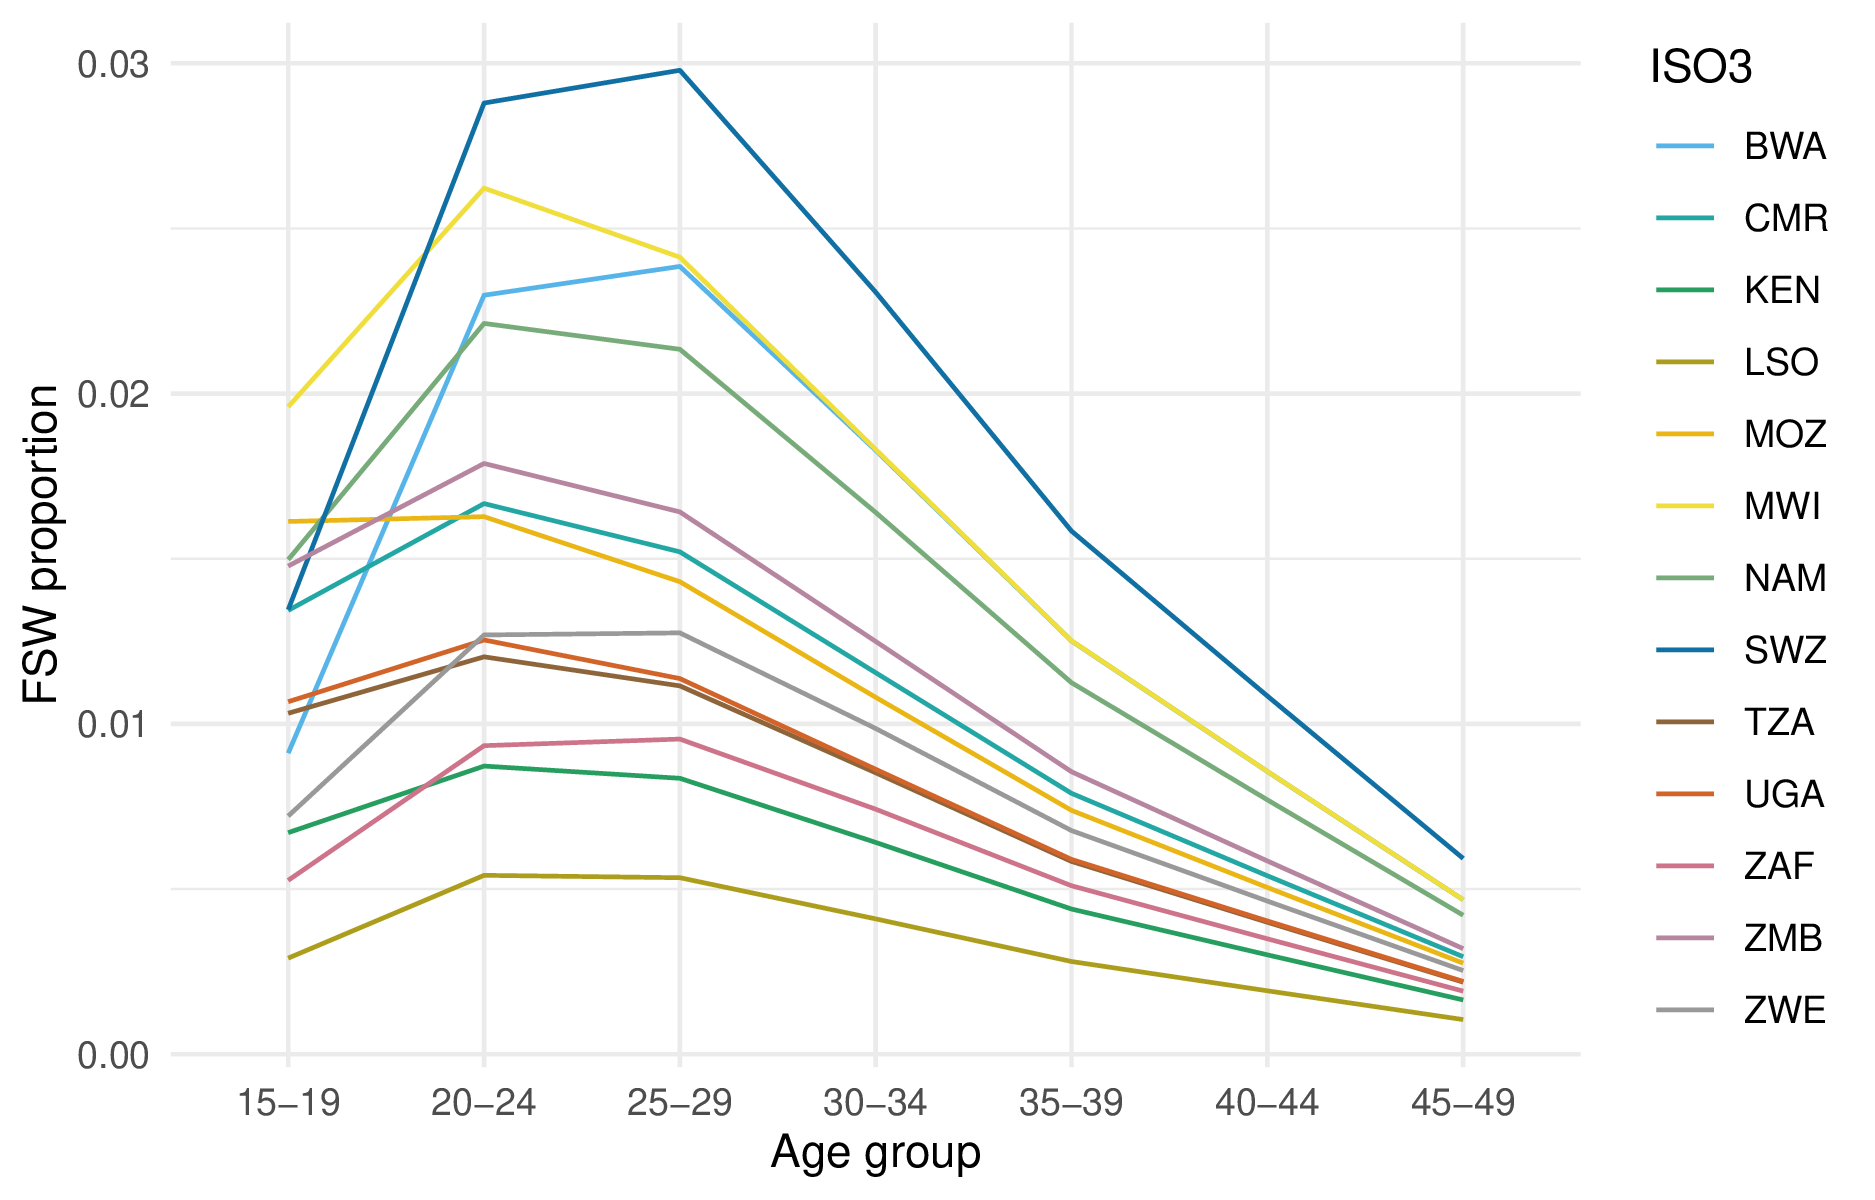
\includegraphics[width=0.9\linewidth]{resources/multi-agyw/20230627-144735-3da88508/depends/age-disagg-fsw-line} 

}

\caption{The disaggregation procedure I used produces a plausible age distirbution of FSW by country.}\label{fig:age-disagg-fsw-line}
\end{figure}

\hypertarget{results-2}{%
\subsection{Results}\label{results-2}}

\hypertarget{coverage-assessment}{%
\subsubsection{Coverage assessment}\label{coverage-assessment}}

To assess the calibration of the fitted model, I calculated the quantile \(q\) of each observation within the posterior predictive distribution.
For calibrated models, these quantiles, known as probability integral transform (PIT) values \autocite{dawid1984present,bosse2022scoringutils}, should follow a uniform distribution \(q \sim \mathcal{U}[0, 1]\).
To generate samples from the posterior predictive distribution, I applied the multinomial likelihood to samples from the latent field, setting the sample size to be the floor of the Kish effective sample size.

Using the PIT values, it is possible to calculate the empirical coverage of all \((1 - \alpha)100\)\% (equal-tailed) posterior predictive credible intervals.
These empirical coverages can be compared to the nominal coverage \((1 - \alpha)\) for each value of \(\alpha \in [0, 1]\) to give empirical cumulative distribution function (ECDF) difference values.
This approach has the advantage of considering all possible confidence values at once.
\textcite{sailynoja2021graphical} develop binomial distribution-based simultaneous confidence bands for ECDF difference values which test uniformity.

\hypertarget{variance-decomposition}{%
\subsubsection{Variance decomposition}\label{variance-decomposition}}

\hypertarget{estimates}{%
\subsubsection{Estimates}\label{estimates}}

\hypertarget{prevalence-and-incidence-by-risk-group}{%
\section{Prevalence and incidence by risk group}\label{prevalence-and-incidence-by-risk-group}}

\hypertarget{disaggregation-of-naomi-estimates}{%
\subsection{Disaggregation of Naomi estimates}\label{disaggregation-of-naomi-estimates}}

I calculated HIV incidence \(\lambda_{iak}\) and number of new HIV infections \(I_{iak}\) stratified according to district, age group and risk group by linear disaggregation
\begin{align}
    I_{ia} &= \sum_k I_{iak} = \sum_k \lambda_{iak}N_{iak} \\
    &= 0 + \lambda_{ia2} N_{ia2} + \lambda_{ia3} N_{ia3} + \lambda_{ia4} N_{ia4} \\
    &= \lambda_{ia2} \left(N_{ia2}  + \text{RR}_{3} N_{ia3} + \text{RR}_4(\lambda_{ia}) N_{ia4}  \right).
\end{align}
Risk group specific HIV incidence estimates are then given by
\begin{align}
    \lambda_{ia1} &= 0, \\
    \lambda_{ia2} &= I_{ia} / \left(N_{ia2} + \text{RR}_{3} N_{ia3} + \text{RR}_4(\lambda_{ia}) N_{ia4}\right), \\
    \lambda_{ia3} &= \text{RR}_{3} \lambda_{ia2}, \\
    \lambda_{ia4} &= \text{RR}_4(\lambda_{ia}) \lambda_{ia2}.
\end{align}
which I evaluated using Naomi model estimates of the number of new HIV infections \(I_{ia} = \lambda_{ia} N_{ia}\), HIV infection risk ratios \(\{\text{RR}_3, \text{RR}_4(\lambda_{ia})\}\), and risk group population sizes as above.
The risk ratio \(\text{RR}_4(\lambda_{ia})\) was defined as a function of general population incidence.
The number of new HIV infections are then \(I_{iak} = \lambda_{iak} N_{iak}\).

\hypertarget{expected-new-infections-reached}{%
\subsection{Expected new infections reached}\label{expected-new-infections-reached}}

I calculated the number of new infections that would be reached prioritising according to each possible stratification of the population--that is for all \(2^3 = 8\) possible combinations of stratification by location, age, and risk group.
As an illustration, for stratification just by age, I aggregated the number of new HIV infections and HIV incidence as such
\begin{align}
    I_a &= \sum_{ik} I_{iak}, \\
    \lambda_a &= I_a / \sum_{ik} N_{iak}.
\end{align}
Under this stratification, individuals in each age group \(a\) are prioritised according to the highest HIV incidence \(\lambda_a\).
By cumulatively summing the expected infections, for each fraction of the total population reached I calculated the fraction of total expected new infections that would be reached.

\hypertarget{results-3}{%
\subsection{Results}\label{results-3}}

\hypertarget{discussion-1}{%
\section{Discussion}\label{discussion-1}}

I estimated the proportion of AGYW who fall into different risk groups at a district level in 13 sub-Saharan African countries.
These estimates support consideration of differentiated prevention programming according to geographic locations and risk behaviour, as outlined in the Global AIDS Strategy.
Systematic differences in risk by age groups, and variation within and between countries, explained the large majority of variation in risk group proportions.
Changes over time were negligible in the overall variation in risk group proportions.
The proportion of 15-19 year olds who are sexually active, and among women aged 20-29 years, norms around cohabitation especially varied across districts and countries.
This variation underscores the need for these granular data to implement HIV prevention options aligned to local norms and risk behaviours.

I considered four risk groups based on sexual behaviour, the most proximal determinant of risk.
Other factors, such as condom usage or type of sexual act, may account for additional heterogeneity in risk from sexual behaviour.
However, I did not include these factors in view of measurement difficulties, concerns about consistency across contexts, and the operational benefits of describing risk parsimoniously.
Sexual behaviour confers risk only when AGYW reside in geographic locations where there is unsuppressed viral load among their potential partners.
I did not include more distal determinants, such as school attendance, orphanhood, or gender empowerment, as I expect their effects on risk to largely be mediated by more proximal determinants.
However, to effectively implement programming, it is crucial to understand these factors, as well as the broader structural barriers and limits to personal agency faced by AGYW.
Importantly, programs must ensure that intervention prioritisation occurs without stigmatising or blaming AGYW.

Brugh et al. \autocite{brugh2021characterizing} previously geographically mapped AGYW HIV risk groups using biomarker and behavioural data from the most recent surveys in Eswatini, Haiti and Mozambique to define and subsequently map risk groups with a range of machine learning techniques.
My work builds on Brugh et al. \autocite{brugh2021characterizing} by including more countries, integrating a greater number of surveys, and connecting risk group proportions with HIV epidemic indicators to help inform programming.

By considering a range of possible risk stratification strategies, I showed that successful implementation of a risk-stratified approach would allow substantially more of those at risk for infections to be identified before infection occurs.
A considerable proportion of estimated new infections were among FSW, supporting the case for HIV programming efforts focused on key population groups \autocite{baral2012burden}.
There is substantial variation in the importance of prioritisation by age, location and behaviour within each country.
This highlights the importance of understanding and tailoring HIV prevention efforts to country-specific contexts.
By standardising our analysis across all 13 countries, I showed the additional efficiency benefits of resource allocation between countries.

I found a geographic delineation in the proportion of women cohabiting between southern and eastern Africa, calling attention to a divide attributable to many cultural, social, and economic factors.
The delineation does not represent a boundary between predominately Christian and Muslim populations, which is further north.
I also note that the high numbers of adolescent girls aged 15-19 cohabiting in Mozambique is markedly different from the other countries \autocite{unicef}.

My modelled estimates of risk group proportions improve upon direct survey results for three reasons.
First, by taking a modular modelling approach, I integrated all relevant survey information from multiple years, allowing estimation of the FSW proportion for surveys without a specific transactional sex question.
Second, whereas direct estimates exhibit large sampling variability at a district level, I alleviated this issue using spatio-temporal smoothing.
Third, I provided estimates in all district-years, including those not directly sampled by surveys, allowing estimates to be consistently fed into further analysis and planning pipelines (such as our analysis of risk group specific prevalence and incidence).

The final surveys included in our risk model model were conducted in 2018.
The analysis may be updated with more surveys as they become available.
I do not anticipate that the risk group proportions will change substantially, as I found that they did not change significantly over time.

My analysis focused on females aged 15-29 years, and could be extended to consider optimisation of prevention more broadly, accounting for the 0\% of new infections among adults 15-49 which occur in women 30-49 and men 15-49.
Estimating sexual risk behaviour in adults 15-49 would be a crucial step toward greater understanding of the dynamics of the HIV epidemic in sub-Saharan Africa, and would allow incidence models to include stratification of individuals by sexual risk.

Phylogenetic results from BDI are about transmission rather than incidence.
Only age-sex structured not age-sex-behaviour.
Does not undermine my work.

\hypertarget{limitations-1}{%
\subsection{Limitations}\label{limitations-1}}

My analysis was subject to challenges shared by most approaches to monitoring sexual behaviour in the general population \autocite{cleland2004monitoring}.
In particular, under-reporting of higher risk sexual behaviours among AGYW could affect the validity of my risk group proportion estimates.
Due to social stigma or disapproval, respondents may be reluctant to report non-marital partners \autocite[\textcite{helleringer2011reliability}]{nnko2004secretive} or may bias their reporting of sexual debut \autocite{zaba2004age,wringe2009comparative,nguyen2022trends}.
For guidance of resource allocation, differing rates of under-reporting by country, district, year or age group are particularly concerning to the applicability of my results; and, while it may be reasonable to assume a constant rate over space-time, the same cannot be said for age, where aspects of under-reporting have been shown to decline as respondents age \autocite{glynn2011assessing}, suggesting that the elevated risks I found faced by younger women are likely a conservative estimate.
If present, these reporting biases will also have distorted the estimates of infection risk ratios and prevalence ratios I used in my analysis, likely over-attributing risk to higher risk groups.

I have the least confidence in my estimates for the FSW risk group.
As well as having the smallest sample sizes, my transactional sex estimates do not overcome the difficulties of sampling hard to reach groups.
I inherent any limitations of the national FSW estimates \autocite{stevens2022estimating} which I adjust my estimates of transactional sex to match.
Furthermore, I do not consider seasonal migration patterns, which may particularly affect FSW size.
More generally, I did not consider covariates potentially predictive of risk group proportions (such as sociodemographic characteristics, education, local economic activity, cultural and religious norms and attitudes), which are typically difficult to measure spatially.
Identifying measurable correlates of risk, or particular settings in which time-concentrated HIV risk occurs, is an important area for further research to improve risk prioritisation and precision HIV programme delivery.

The efficiency of each stratified prevention strategy depends on the ability of programmes to identify and effectively reach those in each strata.
My analysis of new infections potentially averted assumed a ``best-case'' scenario where AGYW of every strata can be reached perfectly, and should therefore be interpreted as illustrating the potentially obtainable benefits rather than benefits which would be obtained from any specific intervention strategy.
In practice, stratified prevention strategies are likely to be substantially less efficient than this best-case scenario.
Factors I did not consider include the greater administrative burden of more complex strategies, variation in difficulty or feasibility of reaching individuals in each strata, variation in the range or effectiveness of interventions by strata, and changes in strata membership that may occur during the course of a year.
Identifying and reaching behavioural strata may be particularly challenging.
Empirical evaluations of behavioural risk screening tools have found only moderate discriminatory ability \autocite{jia2022risk}, and risk behaviour may change rapidly among young populations, increasing the challenge to effectively deliver appropriately timed prevention packages.
This consideration may motivate selecting risk groups based on easily observable attributes, such as attendance of a particular service or facility, rather than sexual behaviour.

I did not engage with country experts or civil society organisations.
This led to problems, including in Malawi.
Future work should be better.

\hypertarget{conclusion-1}{%
\subsection{Conclusion}\label{conclusion-1}}

I estimated the proportion of AGYW aged 15-19, 20-24 and 25-29 years in four sexual risk groups at a district-level in 13 priority countries and analyzed the number of infections that could be reached by prioritisation based upon location, age and behaviour.
Though subject to limitations, these estimates provide data that national HIV programmes can use to set targets and implement differentiated HIV prevention strategies as outlined in the Global AIDS Strategy.
Successfully implementing this approach would result in more efficiently reaching a greater number of those at risk of infection.

Among AGYW, there was systematic variation in sexual behaviour by age and location, but not over time.
Age group variation was primarily attributable to age of sexual debut (ages 15-24).
Spatial variation was particularly present between those who reported one cohabiting partner versus non-regular or multiple partners.
Risk group proportions did not change substantially over time, indicating that norms relating to sexual behaviour are relatively static.
These findings underscore the importance of providing effective HIV prevention options tailored to the needs of particular age groups, as well as local norms around sexual partnerships.

\hypertarget{naomi-aghq}{%
\chapter{Fast approximate Bayesian inference}\label{naomi-aghq}}

\adjustmtc
\markboth{Fast, approximate inference for the Naomi model}{}

In this chapter I describe a novel Bayesian inference method I developed with the aim of facilitating fast and accurate inference for the Naomi small-area estimation model.
Naomi is a complex model, used in over 35 countries in sub-Saharan Africa to produce estimates of HIV indicators.
The results are presented in \textcite{howes2023fast}.

Though I began working on this project in 2020, I only started to make significant progress after reading \textcite{stringer2021fast}.
I am grateful to have subsequently collaborate with Alex Stringer on this project, including my visiting the University of Waterloo during the fall term of 2022.

Code for the analysis in this chapter is available from \href{https://github.com/athowes/elgm-inf}{\texttt{athowes/naomi-aghq}} and supported by the R package \href{https://athowes.github.io/inf.utils}{\texttt{inf.utils}}.

\hypertarget{background-3}{%
\section{Background}\label{background-3}}

The goal of a Bayesian analysis is to obtain the posterior distribution \(p(\bvartheta \, | \, \y)\).
This is a reasonable goal because given a loss function \(L\), the posterior loss of action \(a\) depends on the data only via the posterior distribution.
It is usually intractable to directly obtain the posterior distribution, because the denominator contains the integral
\begin{equation}
p(\y) = \int_{\mathbb{R}^d} p(\y, \bvartheta) \text{d}\bvartheta
\end{equation}
As such, approximations to the posterior distribution are typically used.

\hypertarget{inference-methods}{%
\section{Inference methods}\label{inference-methods}}

\hypertarget{the-laplace-approximation}{%
\subsection{The Laplace approximation}\label{the-laplace-approximation}}

The posterior normalising constant may be approximated using Laplace's method \autocite{tierney1986accurate}.
Let \(h(\bvartheta) = \log p(\bvartheta, \y)\) such that
\begin{equation}
p(\y) = \int_{\mathbb{R}^d} p(\y, \bvartheta) \text{d}\bvartheta = \int_{\mathbb{R}^d} \exp(h(\bvartheta)) \text{d}\bvartheta.
\end{equation}
Let
\begin{equation}
\hat \bvartheta = \argmax_{\bvartheta} h(\bvartheta)
\end{equation}
be the posterior mode, and
\begin{equation}
\hat {\Hb} = - \frac{\partial^2}{\partial \bvartheta \partial \bvartheta^\top} h(\bvartheta) \rvert_{\bvartheta = \hat \bvartheta}
\end{equation}
be the Hessian matrix evaluated at the posterior mode.
Taking a second order Taylor approximation at the posterior mode gives the Laplace approximation to the normalising constant as
\begin{align}
\tilde p_{\texttt{LA}}(\y) &= \int_{\mathbb{R}^d} \exp \left( h(\hat \bvartheta) - \frac{1}{2} (\bvartheta - \hat \bvartheta)^\top \hat {\Hb} (\bvartheta - \hat \bvartheta) \right) \text{d}\bvartheta \label{eq:la} \\
&= \exp(h(\hat \bvartheta)) \cdot \frac{(2 \pi)^{d/2}}{| \hat {\Hb} |^{1/2}},
\end{align}
where Equation \ref{eq:la} is calculated using the normalising constant of the Gaussian distribution \(\mathcal{N}(\cdot \, | \, \hat \bvartheta, \hat {\Hb}^{-1})\).

\hypertarget{adaptive-gauss-hermite-quadrature}{%
\subsection{Adaptive Gauss-Hermite quadrature}\label{adaptive-gauss-hermite-quadrature}}

Another way to approximate the posterior normalising constant is using quadrature.
Let \(\mathcal{Q}\) be a set of quadrature points, and \(\omega: \mathbb{R}^d \to \mathbb{R}\) be a weighting function.
Then a quadrature approximation to the posterior normalising constant is given by
\begin{equation}
\tilde p(\y) = \sum_{\bvartheta \in \mathcal{Q}} p(\y, \bvartheta) \omega(\bvartheta).
\end{equation}

\hypertarget{integrated-nested-laplace-approximation}{%
\subsection{Integrated nested Laplace approximation}\label{integrated-nested-laplace-approximation}}

\hypertarget{a-universal-inla-implementation}{%
\section{A universal INLA implementation}\label{a-universal-inla-implementation}}

In this section, I implement the INLA method from scratch, using the \texttt{TMB} package.
The result is universal in that it is compatible with any model with a \texttt{TMB} C++ template for the log-posterior.
The \texttt{R-INLA} software uses a formula interface (e.g.~\texttt{y\ \textasciitilde{}\ 1\ +\ x}) which facilitates use of the method for common models.
Though beneficial for new users, this imposes constraints on advanced users who would like to use more complicated models.
Indeed \textcite{martino2019integrated} note that ``implementing INLA from scratch is a complex task'', and as a result ``applications of INLA are limited to the (large class of) models implemented {[}in \texttt{R-INLA}{]}''.
\textcite{skaug2009approximate} highlights the potential benefits of a more flexible INLA implementation using automatic differentiation.

I demonstrate the implementation using the epilepsy generalised linear mixed model example from \textcite{spiegelhalter1996bugs}.
The model is based on that of \textcite{breslow1993approximate}, itself a modification of \textcite{thall1990some}, and the data are from an epilespy drug double-blind clinical trial \autocite{leppik1985double}.
\textcite{rue2009approximate} (Section 5.2) demonstrate the INLA method using this example, and find that there is a difference in approximation error depending on use of either the Gaussian or Laplace approximation for some parameters (Figure 3).

In the trial, patients \(i = 1, \ldots, 59\) were each assigned either the new drug \(\texttt{Trt}_i = 1\) or placebo \(\texttt{Trt}_i = 0\).
Each patient made four visits the clinic \(j = 1, \ldots, 4\), and the observations \(y_{ij}\) are the number of seizures of the \(i\)th person in the two weeks preceding their \(j\)th visit.
The covariates used in the model were age \(\texttt{Age}_i\), baseline seizure counts \(\texttt{Base}_i\) and an indicator for the final clinic visit \(\texttt{V}_4\), which were all centered.
The observations were modelled using a Poisson distribution \(y_{ij} \sim \text{Poisson}(e^{\eta_{ij}})\) with linear predictor
\begin{align*}
\eta_{ij}
&= \beta_0 + \beta_\texttt{Base} \log(\texttt{Baseline}_j / 4) + \beta_\texttt{Trt} \texttt{Trt}_i +
   \beta_{\texttt{Trt} \times \texttt{Base}} \texttt{Trt}_i \times \log(\texttt{Baseline}_j / 4) \\ 
&+ \beta_\texttt{Age} \log(\texttt{Age}_i) + \beta_{\texttt{V}_4} {\texttt{V}_4}_j +
   \epsilon_i + \nu_{ij}, \quad i \in [59], \quad j \in [4],
\end{align*}
where the prior distribution on each of the regression parameters, including the intercept, was \(\mathcal{N}(0, 100^2)\).
The random effects are IID \(\epsilon_i \sim \mathcal{N}(0, 1/\tau_\epsilon)\) and \(\nu_{ij} \sim \mathcal{N}(0, 1/\tau_\nu)\) with precision prior distributions \(\tau_\epsilon, \tau_\nu \sim \Gamma(0.001, 0.001)\).

\hypertarget{naomi-model}{%
\section{Naomi model}\label{naomi-model}}

\hypertarget{malawi-case-study}{%
\section{Malawi case-study}\label{malawi-case-study}}

\hypertarget{discussion-2}{%
\section{Discussion}\label{discussion-2}}

\hypertarget{conclusions}{%
\chapter{Future work and conclusions}\label{conclusions}}

\adjustmtc
\markboth{Conclusions}{}

\hypertarget{strengths}{%
\section{Strengths}\label{strengths}}

\hypertarget{chapter-refbeyond-borders}{%
\subsection{Chapter \ref{beyond-borders}}\label{chapter-refbeyond-borders}}

\begin{itemize}
\tightlist
\item
  I designed experiments to thoroughly compare models for spatial structure using tools for model assessment such as proper scoring rules and posterior predictive checks.
\end{itemize}

\hypertarget{chapter-refmulti-agyw}{%
\subsection{Chapter \ref{multi-agyw}}\label{chapter-refmulti-agyw}}

\begin{itemize}
\tightlist
\item
  I estimated HIV risk group proportions for AGYW, enabling countries to prioritise their delivery of HIV prevention services.
\item
  I analysed the number of new infections that might be reached under a variety of risk stratification strategies.
\item
  I used \texttt{R-INLA} to specify multinomial spatio-temporal models via the Poisson-multinomial transformation. This includes complex two- and three-way Kronecker product interactions defined using the \texttt{group} and \texttt{replicate} options.
\end{itemize}

\hypertarget{chapter-refnaomi-aghq}{%
\subsection{Chapter \ref{naomi-aghq}}\label{chapter-refnaomi-aghq}}

\begin{itemize}
\tightlist
\item
  I developed a novel Bayesian inference method, motivated by a challenging and practically important problem in HIV inference.
\item
  The method enables integrated nested Laplace approximations to be fit to and studied on a wider class of models than was previously possible.
\item
  My implementation of the method was straightforward, building on the \texttt{TMB} and \texttt{aghq} packages, and described completely and accessibly in \textcite{howes2023fast}.
\end{itemize}

\hypertarget{future-work}{%
\section{Future work}\label{future-work}}

Avenues for future work include:

\begin{enumerate}
\def\labelenumi{\arabic{enumi}.}
\tightlist
\item
  Extending the risk group model described in Chapter \ref{multi-agyw} to include all adults 15-49. This may involve modelling of age-stratified sexual partnerships \autocite{wolock2021evaluating}.
  Such a model would likely fall out of the scope of \texttt{R-INLA}, but would be possible to write with \texttt{TMB} and therefore amenable to the methods discussed in Chapter \ref{naomi-aghq}.
\item
  Speeding up the implementation of Laplace marginals using the matrix algebra approximations described in \textcite{wood2020simplified}.
\item
  Evaluating the accuracy of deterministic Bayesian inference methods for a broader variety of extended latent Gaussian models.
\end{enumerate}

\hypertarget{conclusions-1}{%
\section{Conclusions}\label{conclusions-1}}

\begin{itemize}
\tightlist
\item
  Modelling complex data, more often than not, pushes the boundaries of the statistical toolkit available.
\item
  A challenge I encountered was the difficulty of implementing identical models across multiple frameworks with the aim of studying the inference method. Or, of a similarly fraught nature, comparing different models implemented in different frameworks with the aim of studying model differences. The frequently asked questions section of the \texttt{R-INLA} website \autocite{rinla2023faq} notes that ``the devil is in the details''. I have resolved this challenge by using a given \texttt{TMB} model template to fit models using multiple inference methodologies. The benefits of such a ecosystem of packages are noted by \textcite{stringer2021fields}. I particularly highlight the benefit of enabling analysts to easily vary their choice of inference method based on the stage of model development that they are in.
\item
  To the best of my abilities, I have written this thesis, and the work described within it, in keeping with the principles of open science. I hope that doing so allows my work to be scrutinised, and optimistically built upon. This would not have been possible without a range of tools from the R ecosystem such as \texttt{rmarkdown} and \texttt{rticles}, as well as those developed within the MRC Centre for Global Infectious Disease Analysis such as \texttt{orderly} and \texttt{didehpc}.
\end{itemize}

\startappendices

\hypertarget{spatial-structure-supplement}{%
\chapter{Spatial structure supplement}\label{spatial-structure-supplement}}

\hypertarget{a-model-for-risk-group-proportions-supplement}{%
\chapter{A model for risk group proportions supplement}\label{a-model-for-risk-group-proportions-supplement}}

\hypertarget{fast-approximate-bayesian-inference-supplement}{%
\chapter{Fast approximate Bayesian inference supplement}\label{fast-approximate-bayesian-inference-supplement}}


%%%%% REFERENCES

% JEM: Quote for the top of references (just like a chapter quote if you're using them).  Comment to skip.
% \begin{savequote}[8cm]
% The first kind of intellectual and artistic personality belongs to the hedgehogs, the second to the foxes \dots
%   \qauthor{--- Sir Isaiah Berlin \cite{berlin_hedgehog_2013}}
% \end{savequote}

\setlength{\baselineskip}{0pt} % JEM: Single-space References

{\renewcommand*\MakeUppercase[1]{#1}%
\printbibliography[heading=bibintoc,title={\bibtitle}]}


\end{document}
